% MODEL THESIS FILE
% This is the file to typeset. It then imports the other .tex files to be typeset.

\documentclass[12pt,oneside, reqno]{amsbook}
\usepackage{epsfig}
\usepackage{setspace} 
\usepackage{minted}
\setstretch{1.5}


%shortcut commands
\newcommand{\beq}{\begin{equation}}
\newcommand{\eeq}{\end{equation}}
\newcommand{\Zeta}{\mathrm{Z}}


%this sets the margins to 1" on all sides -- the amsbook gives giant margins.
\addtolength{\oddsidemargin}{-.875in}
\addtolength{\evensidemargin}{-.875in}
\addtolength{\textwidth}{1.75in}

\addtolength{\topmargin}{-.5in}
\addtolength{\textheight}{1in}


% above is the preamble


%\renewcommand{\baselinestretch}{2} %Use this for double-spacing.
\usepackage{graphicx} % You need graphicx for importing graphics files.

\numberwithin{equation}{chapter}
% This numbers the equations within each chapter as 1.1, 1.2, 2.1, etc.
\numberwithin{figure}{chapter}
% This does the same for the figures.

\theoremstyle{plain} % This is the default style.
\newtheorem{thm}{Theorem}[chapter]
\newtheorem{cor}[thm]{Corollary}
\newtheorem{prop}[thm]{Proposition}
\newtheorem{lem}[thm]{Lemma}
% [chapter] causes the above to be numbered within each chapter as 1.1, 1.2, ...
% If you omit [chapter], the numbers will be 1, 2, ...

\theoremstyle{definition}
\newtheorem*{dfn}{Definition}
% The asterisk suppresses the numbering of definitions.

\theoremstyle{remark}
\newtheorem{ex}{Example}
\newtheorem*{rem}{Remark}
% The asterisk suppresses the numbering of remarks.

\graphicspath{{converted_graphics/}}





\begin{document}

\frontmatter % Pages here will be numbered with Roman numerals.
\title[]{Optical Pumping of Rubidium Atoms to form Bose-Einstein Condensation}
\author{Adrian Miguel deCola}
\address{Department of Physics and Astronomy \\Bates College\\Lewiston, ME 04240}
\date{April 17, 2023}
\maketitle

% Create real cover page.
\newpage
\thispagestyle{empty} 			% Suppress numbering of this page.
% THESIS COVER PAGE

% Choose Honors/Senior and Arts/Science below as appropriate.

\vspace*{4cm} 
% LaTeX will remove blank space at the start or end of a page,
%   but the asterisk prevents this.

\centerline{\LARGE \textbf{Optical Pumping of Rubidium Atoms}}
\medskip
\centerline{\LARGE \textbf{  to form Bose-Einstein Condensation }} 
\medskip
\begin{figure}[h!]
\begin{center}

\epsfig{file=fig_bates.png, scale = .1195}
\end{center}
\end{figure}
\centerline{ A Senior Thesis}
\medskip
\centerline{ Presented to the Department of Physics and Astronomy}
\medskip
\centerline{Bates College}
\medskip
\centerline{in partial fulfillment of the requirements for the}
\medskip
\centerline{\Large Degree of Bachelor of Science}
\medskip
\centerline{by}
\medskip
\centerline{\Large Adrian Miguel deCola}
\medskip
\centerline{Lewiston, Maine}
\medskip
\centerline{April 17, 2023}

\newpage

       			% Save the file cover.tex to the same folder as thesis.tex.
\setcounter{page}{2}




\tableofcontents
% This creates a file called thesis.toc.

% \listoftables
% \listoffigures
% Use the above if you have tables/figures and want them listed in the front.

% The following files should be in the same folder as thesis.tex.



\chapter*{Acknowledgments}
% The asterisk prevents this file from being labelled
% as a 'chapter.'

I would like to express my thanks to my mom for her support, love, and encouragement throughout my academic journey. Thank you for always being there for me. Her support, guidance, and encouragement have been invaluable to me. I am extremely grateful for her sacrifices to support me. 


I would also like to thank my advisor, Nathan Lundblad, for his guidance and instruction. His hours of teaching have been extremely valuable to my learning. Thanks to my teachers in the Physics, Computer Science, and Economics departments who have been influential to my learning. I would especially like to extend my gratitude to Hong Lin, who has been been extremely influential in forming my reasoning skills and fostering my interest in Physics. \cite{nlundblad} \cite{hlin}


In addition, I would like to express my sincere appreciation to all the previous researchers whose work and theses gave me a foundation in this project and a learning reference. \cite{sshea}\cite{mcwik}\cite{dpaseltiner}


Finally, I would like to acknowledge the contributions of all the individuals who have supported my personal and academic growth along the way, including my fellow colleagues, friends, and mentors. 




     			% Acknowledgments



\mainmatter % Pages here will be numbered 1, 2, 3, and so on .


\chapter*{Introduction}
% The asterisk prevents this file from being labelled
% as a 'chapter.'

Occasionally referred to as the fifth state of matter, Bose-Einstein Condensation pushes the extremes of our physical universe. Super-cooled to within a millionth of a degree of absolute zero, these particles harmoniously lose their individuality, joining together to form a 'quantum super particle'. This extraordinary state of matter, Bose-Einstein Condensation, pushed the frontier of physics and remains a great example of generational achievement and scientific teamwork. Today, Bose-Einstein Condensation remains a heavily interesting field researched in areas such as supersolids, quantum computers, and precision measurement. 


Against the backdrop of World War I, physicist and mathematician Satyendra Bose sent a paper to Albert Einstein about the statistical relationship between light and temperature, where he treated photons as indistinguishable particles. Einstein, impressed with his work, translated and submitted the paper on his behalf to a physics journal where it was later published. Einstein extended Bose's statistics to indistinguishable atoms, resulting in Bose-Einstein Statistics. These indistinguishable atoms are part of a family of particles called bosons. With this framework, Einstein formulated a state of matter where a cloud of atoms could be cooled enough until they all condense to the same, lowest, quantum state. This new state of matter is what we refer to as Bose-Einstein Condensation. Einstein published his findings in 1925. At the time, he described the state of matter, saying "this appears to be as good as it is impossible." Such a state of matter at the time appeared to many, as nonsensical, with atoms overlapping and all sharing the same properties. 


It wasn't until 70 years later, in 1995, with new advances in laser cooling, magnetic trapping, evaporative cooling, vacuum technology, and theoretical understanding that a Bose-Einstein Condensate was finally realized, using Rubidium atoms much like the Ultra-Cold Atom Lab at Bates. Eric Cornell, Carl Wieman, and Wolfgang Ketterle received the 2001 Nobel Prize in Physics for being the first labs to produce Bose-Einstein Condensates.


In the past 38 year, Bose-Einstein Condensate technology has greatly improved. There are now hundreds of labs around the world with functioning Bose-Einstein Condensate machines. Scientists have made Bose-Einstein Condensates out of many other bosons including Alkali atoms such as Rubidium, Sodium, Cesium, Lithium, and others; noble gasses like Helium-4; and even photons. Bose-Einstein Condensates are especially interesting as they demonstrate quantum behavior on a macroscopic scale, can display unique properties such as super fluidity and coherence, and because of their tunability, which is useful for simulation. Due to these properties, Bose-Einstein Condensates remain among the leading areas of research; especially in condensed matter physics, quantum simulation and information, and precision measurements. 


Over the past years, Nathan Lundblad, Bates students, and post-doctorates have worked to create an atom chip based Bose-Einstein Condensate machine. This atom chip based machine will complement the currently functional Bose-Einstein Condensate machine in the lab. The motivation behind another machine is to build a smaller, lighter, easily controlled Bose-Einstein Condensate machine, much like the one in the Cold Atom Lab on the International Space Station. This new machine will be useful for simulating experiments we hope to perform on the International Space Station. One example of this is the realization of a 'bubble-like' Bose-Einstein Condensate. Creating a magnetic field gradient for a Bose-Einstein Condensate of this shape is not possible in the presence of Earth's gravitational field. Realizing one on the International Space Station has not yet been possible and an atom chip based Bose-Einstein Condensate machine could help in the diagnostics of this quest. An atom chip based Bose-Einstein Condensate machine has the potential to open many other avenues of research with its precise control systems, sleekness, and its utility to simulate experiments on the Cold Atom Lab on the International Space Station. 


This thesis builds upon the work done by previous students. To create a deep, intuitive understanding of the project, this thesis first provides a theoretical framework for which to under Bose-Einstein Condensation and the process for its experimental realization. This thesis works to advances the creation of an optical pumping system to purify the Rubidium-87 atoms into a single substate, $m_F = 2$. The second part of my thesis works to computationally simulate the optical pumping process. This simulation gives a deeper understanding to the process of purifying the atoms. It also serves to provide numerical values to optimizing the laser's time scattering atoms, its necessary frequency detuning, and its intensity. Laser characteristic inputs can be changed and recalculated easily for future lab use. The third part of my thesis works towards creating the optical pumping process in the Ultra-Cold Atom Lab at Bates College. This building process uses optical elements including optical fibers, linear polarizers, beam splitters, quarter-wave plates, mirrors, shutters, many mounts, and other elements. Using these elements, we establish a positive circularly polarized light from a coupled optical fiber mounted closely along the axis of the magnetic coils of the ColdQuanta quadruple coil assembly. 
 
 
 From this point, the laser can be correctly frequency detuned by the amount predicted in my optical pumping simulation. Using the ColdQuanta quadruple coil assembly, all the atoms can be effectively trapped by a magnetic field for further cooling en route to forming a Bose-Einstein Condensate. Lastly, my thesis outlines future steps for students to create a functional Bose-Einstein Condensate machine.


    			% Introduction 

% The following files should also be in the same folder as thesis.tex.
%\documentclass[11pt]{article}
%\usepackage{graphicx}

%\begin{document}

\chapter{Bose-Einstein Condensation}
This chapter explores both a theoretical framework for forming Bose-Einstein Condensation as well as the experimental process on the atom chip based machine. 
\newline

\section{Theoretical Basis for Bose-Einstein Condensation}
This section will discuss the basics of Bose-Einstein statistics, introducing the quantum statistics that describe systems of bosons. Assuming a basis in Boltzmann statistics, the Bose-Einstein distribution is built. From there, the theoretical framework for the realization of Bose-Einstein Condensation will be examined. In this analysis, core concepts for Bose-Einstein Condensate formation will be reviewed including: de Broglie wavelength, critical temperature, and phase space density. 

\subsection{Maxwell-Boltzmann Statistics}
Recalling from Thermal Physics, Boltzmann statistics describe the probability that a particle occupies a state $s$ as
\beq
P_s = \frac{1}{\Zeta_1}e^{-E_s/kT}
\eeq
where $k$ is the Boltzmann constant, $E_s$ is the energy of the particle in state $s$, $\mathrm{Z}$ is the partition function, and $T$ is the temperature of the system. 
\newline
This leads to a partition function of the form 
\beq
\Zeta_1 = \sum_s{e^{-E_s/kT}}
\eeq 
in order to satisfy that the probability of finding the particle in any state is certain.
\beq
\sum_s{P_s}=\sum_s{\frac{1}{\Zeta_1}e^{-E_s/kT}} =\frac{\sum_s{e^{-E_s/kT}}}{\sum_s{e^{-E_s/kT}}}=1
\eeq


Likewise, Boltzmann statistics describe the probability that a system of $n$ particles will be found in state $s$ as 
\beq
P_s(n) = \frac{1}{\mathrm{Z}} e^{-n(\epsilon_s-\mu) /kT}
\eeq
where $k$ is the Boltzmann constant, $\epsilon_s$ is the energy of one particle in state $s$, $\Zeta$ is the partition function, $\mu$ is the chemical potential, and $T$ is the temperature of the system. This derivation comes from considering the entropy of different states of the system with its surroundings.

\subsection{Bose-Einstein Statistics}

Recall that bosons do not obey the Pauli-Exclusion principle. So, unlike fermions, $n$ can be any integer from $0$ to $\infty$. Considering this, we can find the partition function for these indistinguishable particles by making sure the probability of that state being occupied by any possible number of bosons is certain.
$$\mathrm{Z} = \sum_n{e^{-n(\epsilon_s-\mu) /kT}}= 1 + e^{-(\epsilon_s-\mu) /kT} + \left( e^{-(\epsilon_s-\mu) /kT} \right)^2 + ... $$
\beq
\mathrm{Z}= \frac{1}{1- e^{-(\epsilon_s-\mu) /kT}}
\eeq
\newline
The following calculates the average number of bosons in a particular energy state, $\bar{n}_s$,
$$\bar{n}_s = \sum_n{nP_s(n)} $$
\beq
\bar{n}_s = \frac{1}{e^{(\epsilon_s-\mu) /kT}-1}
\eeq
The derivation for this can be found in \textbf{Appendix A.1}. This equation is known as the Bose-Einstein distribution. This equation describes the average number of bosons occupying a given state. In the classical limit, with many particles and lots of energy, where quantization becomes obsolete, a Bose-Einstein distribution is equivalent to a Maxwell-Boltzmann distribution, as expected. However, as Einstein discovered, the two distributions vary drastically for low temperatures where quantum mechanics begins to take effect. 
\newline

\subsection{Bose-Einstein Condensates}

Bose-Einstein Condensation formation occurs when the bosons all cluster towards the ground state. Using the equation for a Bose-Einstein distribution, the average number of atoms in the ground state is 
\beq
\bar{N}_0 = \frac{1}{e^{(\epsilon_0-\mu) /kT}-1}
\eeq
where $\epsilon_0$ is the energy of a boson in the ground state. Evidently, the average number of bosons increases as the temperature decreases. This function is of interest when $N_0$ becomes large. 
An expression for the total number of bosons, is therefore
\beq
N = \sum_s{\frac{1}{e^{(\epsilon_s-\mu) /kT}-1}}
\eeq
Evaluating this sum as a continuous integral and solving it yields a solution only valid for low temperatures below what will be defined as the critical temperature, $T_C$. This evaluation uses $g(\epsilon)$, the density of the states, or the number of particle states per unit of energy, calculated by summing the total energy from each electron. This continuous integration is not valid for the ground state and therefore gives a result for the number of atoms in the excited states\cite{foot}.
%MAYBE PUT THIS DERIVATION IN THE APPENDIX
\beq
N_{excited} = 2.612\left( \frac{2\pi mkT}{h^2} \right)^{\frac{3}{2}}V
\eeq
\beq
T_C = 0.527 \frac{h^2}{2\pi mk}\left( \frac{N}{V} \right)^\frac{2}{3}
\eeq
\textbf{Equation 1.9} describes, for temperatures below the critical temperature, the most amount of bosons that can be in excited states. After which, added bosons, under a constant temperature and volume, will go to the ground state. Therefore, this critical temperature describes when bosons start to cascade towards the ground state. The expression for the number of bosons in the excited states can be rewritten as 
\beq
N_{excited} = \left( \frac{T}{T_C} \right)^\frac{3}{2}N
\eeq
Using this, the number of photons in the ground state can be calculated.
$$N = N_{excited} + N_0$$
\beq 
N_0 = \left( 1 - \left( \frac{T}{T_C} \right)^\frac{3}{2} \right) N
\eeq 
These equations are plotted in \textbf{Figure 1.1}.
\begin{figure}[h]
\begin{center}
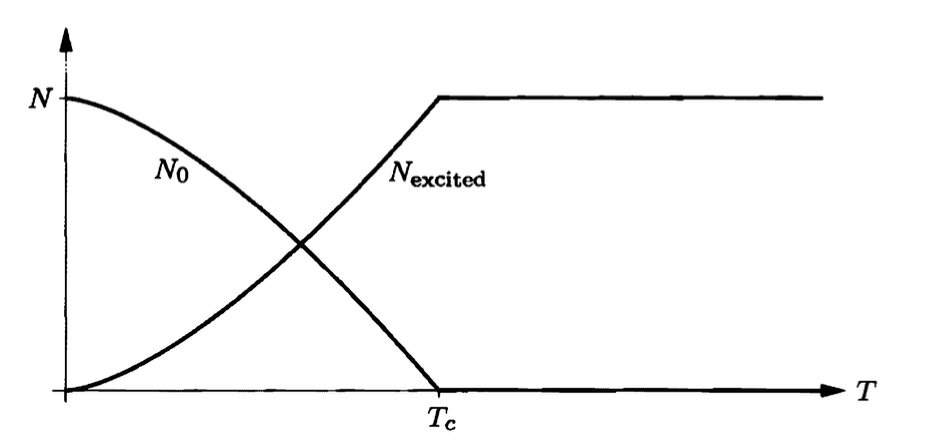
\epsfig{file=fig1_1.png}
\end{center}
\caption{The number of bosons in the excited and ground states.\cite{thermal} }
\end{figure}

Below the critical temperature, the bosons cascade down into the ground state. The number of bosons in the ground state, once below the critical temperature, grows by a factor of $T^{3/2}$ when the temperature decreases. At this point, most bosons share the same quantum state, $\psi$.
%%put figure of first bec from chu and cite?


Another way to think about Bose-Einstein condensation is through the de Broglie wavelength, which describes the wave-like nature of large particles. The thermal de Broglie wavelength, the de Broglie wavelength as a function of temperature, is
\beq 
\lambda_{T} = \frac{h}{\sqrt{2\pi Mk_B T}}
\eeq
At the point of Bose-Einsteins condensation, for Rubidium-87 atoms, like the ones we use in the Ultra-Cold Atom Lab at Bates, the wavelength of the atoms is significantly larger than their spacing or density. This means the wave-functions of the atoms overlap, creating a quantum effect that can be viewed on the scale of the atom cloud, which is about a few millimeters in the Ultra-Cold Lab. Therefore, another way to view the formation of Bose-Einstein condensation is through the phase space density of the bosons, $\rho$. The phase space density can be expressed as
\beq
\rho = n\lambda_T^3
\eeq
where $n$ is the number density of the bosons, or the average distance of a boson to one of its neighbors, and $\lambda_T$ describes the spread of the particles in terms of their wave-like properties. As before, the temperature must be lowered to increase the phase space density. As the thermal de Broglie wavelength grows by a factor of $T^{1/2}$ when the temperature is decreased, the phase space density grows by a factor of $T^{3/2}$. At low enough temperatures, the bosons become indistinguishable, this occurs when they are saturated in the ground state. At this point, the bosons form one 'super particle'. This 'super particle' is the Bose-Einstein Condensate. Its properties are intriguing due to their display of quantum mechanics on a macroscopic scale. Bose-Einstein Condensates can display interesting quantum phenomena such as the uncertainty principles, interference, and quantum tunneling.
\newline



\section{Experimental Process of Forming Bose-Einstein Condensation}

This section will focus on the basic instructions and concepts for forming a Bose-Einstein Condensate on the atom chip based Bose-Einstein Condensation machine in the Bates Ultra-Cold Atom Lab. This machine is referred to as the NASABEC machine due to its eventual goal to simulate experiments similar to the one on the International Space Station. This section will also serve as a basis for understanding the process and the future steps the Ultra-Cold Atom Lab must take. Other labs, including the Ultra-Cold Atom Lab at Bates, use different methods to form Bose-Einstein Condensates and study them. The general steps remain exceedingly similar and this section describes them in order. These general steps include laser cooling, optical pumping and magnetic trapping, and evaporative cooling. This section refrains from an exhaustive mathematical derivation for each step, though the following sources were used to create this section and can be further studied\cite{foot}\cite{metcalf_article}\cite{LCandT}.
\newline

\subsection{Why Rubidium-87?} 

The Ultra-Cold Atom lab uses Rubidium-87 to form Bose-Einstein Condensation. This is due to its unique properties of, of course, being a boson, its stability under low temperatures, and its simple atomic structure. Rubidium-87 has a positive scattering length meaning it is repulsive at low temperatures. Therefore, Rubidium-87 can be confined at low temperatures. Atoms with a negative scattering length, like the more abundant Rubidium-85 would be attracted to each other at these temperatures, violently colliding, and being sent out of the trap. 


In addition to a negative scattering length, Rubidium-87, and many other alkali metals, remain a vapour at these extremely low temperatures required to form a Bose-Einstein Condensate, which was long doubted by scientists. The process of Rubidium-87 forming a metal occurs on a time scale much longer than that necessary to form a Bose-Einstein Condensate. 


The final reason for using Rubidium-87 in Bose-Einstein Condensation formation is due to its simple atomic level structure. Rubidium-87 only has one valence electron. This makes its energy level structure quite simple for the purpose of exciting the valence electron. In addition, the transition of interest, $| F=2\rangle \rightarrow | F=3\rangle$, is a transition with an energy level difference that is quite easy to get relatively cheap lasers for. 


\subsection{Laser Cooling}

Laser cooling is the process of using a laser to drive transitions in atoms and using the recoil energy to slow the atom. Laser cooling uses concepts such as the Doppler effect, the Zeeman effect, and the energy structure of the Rubidium-87 atoms. Laser cooling is the first step in the process of cooling the atoms. To get Rubidium vapor, a piece of Rubidium metal is heated so that atoms sublimate off to be laser cooled. 

The basics behind laser cooling is to use the momentum of many photons to slow down an atom to a limit on the order of the momentum of the photons. On average, the force of one scatter on an atom is equal to the momentum of the absorbed photon. This is because the atom can release the absorbed photon in any direction which, on average, results in a net zero change in momentum for the atom.
\beq
F_{rad} = \frac{IA}{c}
\eeq
The scattering rate for a single atom is given by 
\beq
R_{scatt} = \frac{\Gamma}{2} \frac{\frac{I}{I_{sat}}}{1 + \frac{I}{I_{sat}} + 4 \left( \frac{\delta}{\Gamma}\right)^2 } 
\eeq
\beq 
F_{scatt} = \hbar k  \frac{\Gamma}{2} \frac{\frac{I}{I_{sat}}}{1 + \frac{I}{I_{sat}} + 4 \left( \frac{\delta}{\Gamma}\right)^2 } 
\eeq

where $\Gamma$ is the natural linewidth associated with the excited state, $I$ is the intensity of the laser, $I_{sat}$ is the saturation intensity defined by the transition the atom is being driven between, $k$ is the wave number of the light, and $\delta$ is the frequency detuning of the laser light from the resonant frequency, or the frequency that define the energy level difference in the transition the atom is being driven between. From \textbf{Equation 1.16} it is clear that increasing the intensity of the laser increases the scattering rate, though there is a maximum scattering rate of $\frac{\Gamma}{2}$ as the intensity approaches infinity. For this reason, lasers with output intensities much larger than the saturation intensity are not significantly more beneficial, making them undesired due to their steep costs. 


The frequency detuning can be expressed as
\beq
\delta = \omega - \omega_0 + k \nu
\eeq
where $\omega$ is the frequency of the light coming from the laser, $\omega_0$ is the resonant frequency for the transition, and $k\nu$ is the frequency shift of the light due to the Doppler effect. $k$ is the wave-number of the radiation, and $\nu$ is the velocity of the atom. The Doppler shift must be taken into account, because as atom are slowed, the original frequency they saw becomes off resonance; therefore, absorptions and further cooling becomes infeasible. This is discussed further in the context of the NASABEC machine later.  


To slow atoms, one might consider a pairs of orthogonal, counter-propagating beams as shown in \textbf{Figure 1.2}. One might red-detune the laser frequencies ($\omega < \omega_0$) so that atoms moving toward a laser, due to the Doppler shift, will be more likely to scatter light. This set up provides what is known as optical molasses. A set up of optical molasses is shown in \textbf{Figure 1.2}


\begin{figure}[h!]
\begin{center}
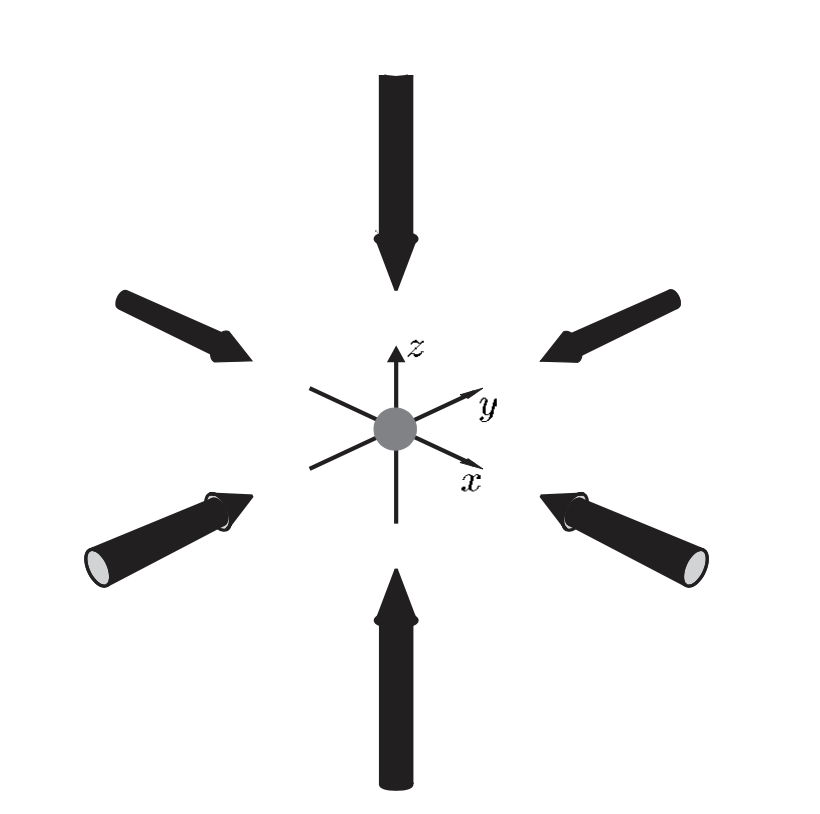
\epsfig{file=fig_optical_molasses.png, scale = .5}
\end{center}
\caption{An set up to create optical molasses.\cite{foot} }
\end{figure}

It is intuitive, since the forces here are velocity dependent, that the result will be a dampening force. This is true and derived in \cite{foot} and \cite{metcalf_article}.
\beq
F_{molasses} = -\beta \nu
\eeq
where the dampening coefficient is of the form
\beq
\beta = 4 \hbar k^2 \frac{I}{I_{sat}} \frac{-2\delta / \Gamma }{\left( 1 + (2\delta / \Gamma )^2 \right)^2}
\eeq

This is a problem if we plan on running this for a long time. This is because the atoms feel no central restoring force. Atoms will leave the optical molasses, hit the side of the structure that encloses them in a vacuum and heat up. For this reason, optical molasses is used for a short period of time once the gas has been cooled to the order of about $100\mu K$. This step in cooling takes advantage of the hyperfine structure of Rubidium-87. \cite{foot}\cite{metcalf_article}\cite{LCandT}

To apply a central restoring force, a magneto-optical trap is used. To build a magneto-optical trap, a magnetic field gradient is applied. This magnetic field splits the energy levels of Rubidium-87 due to the Zeeman effect. This magnetic field, in the NASABEC machine, is formed using quadrupole coils; such that, the strength of the Zeeman splitting, close to the center of the trap, grows as the atoms leave the center of the trap. This splitting for Rubidium-87 can be shown below in \textbf{Figure 1.3}.

\begin{figure}[h!]
\begin{center}
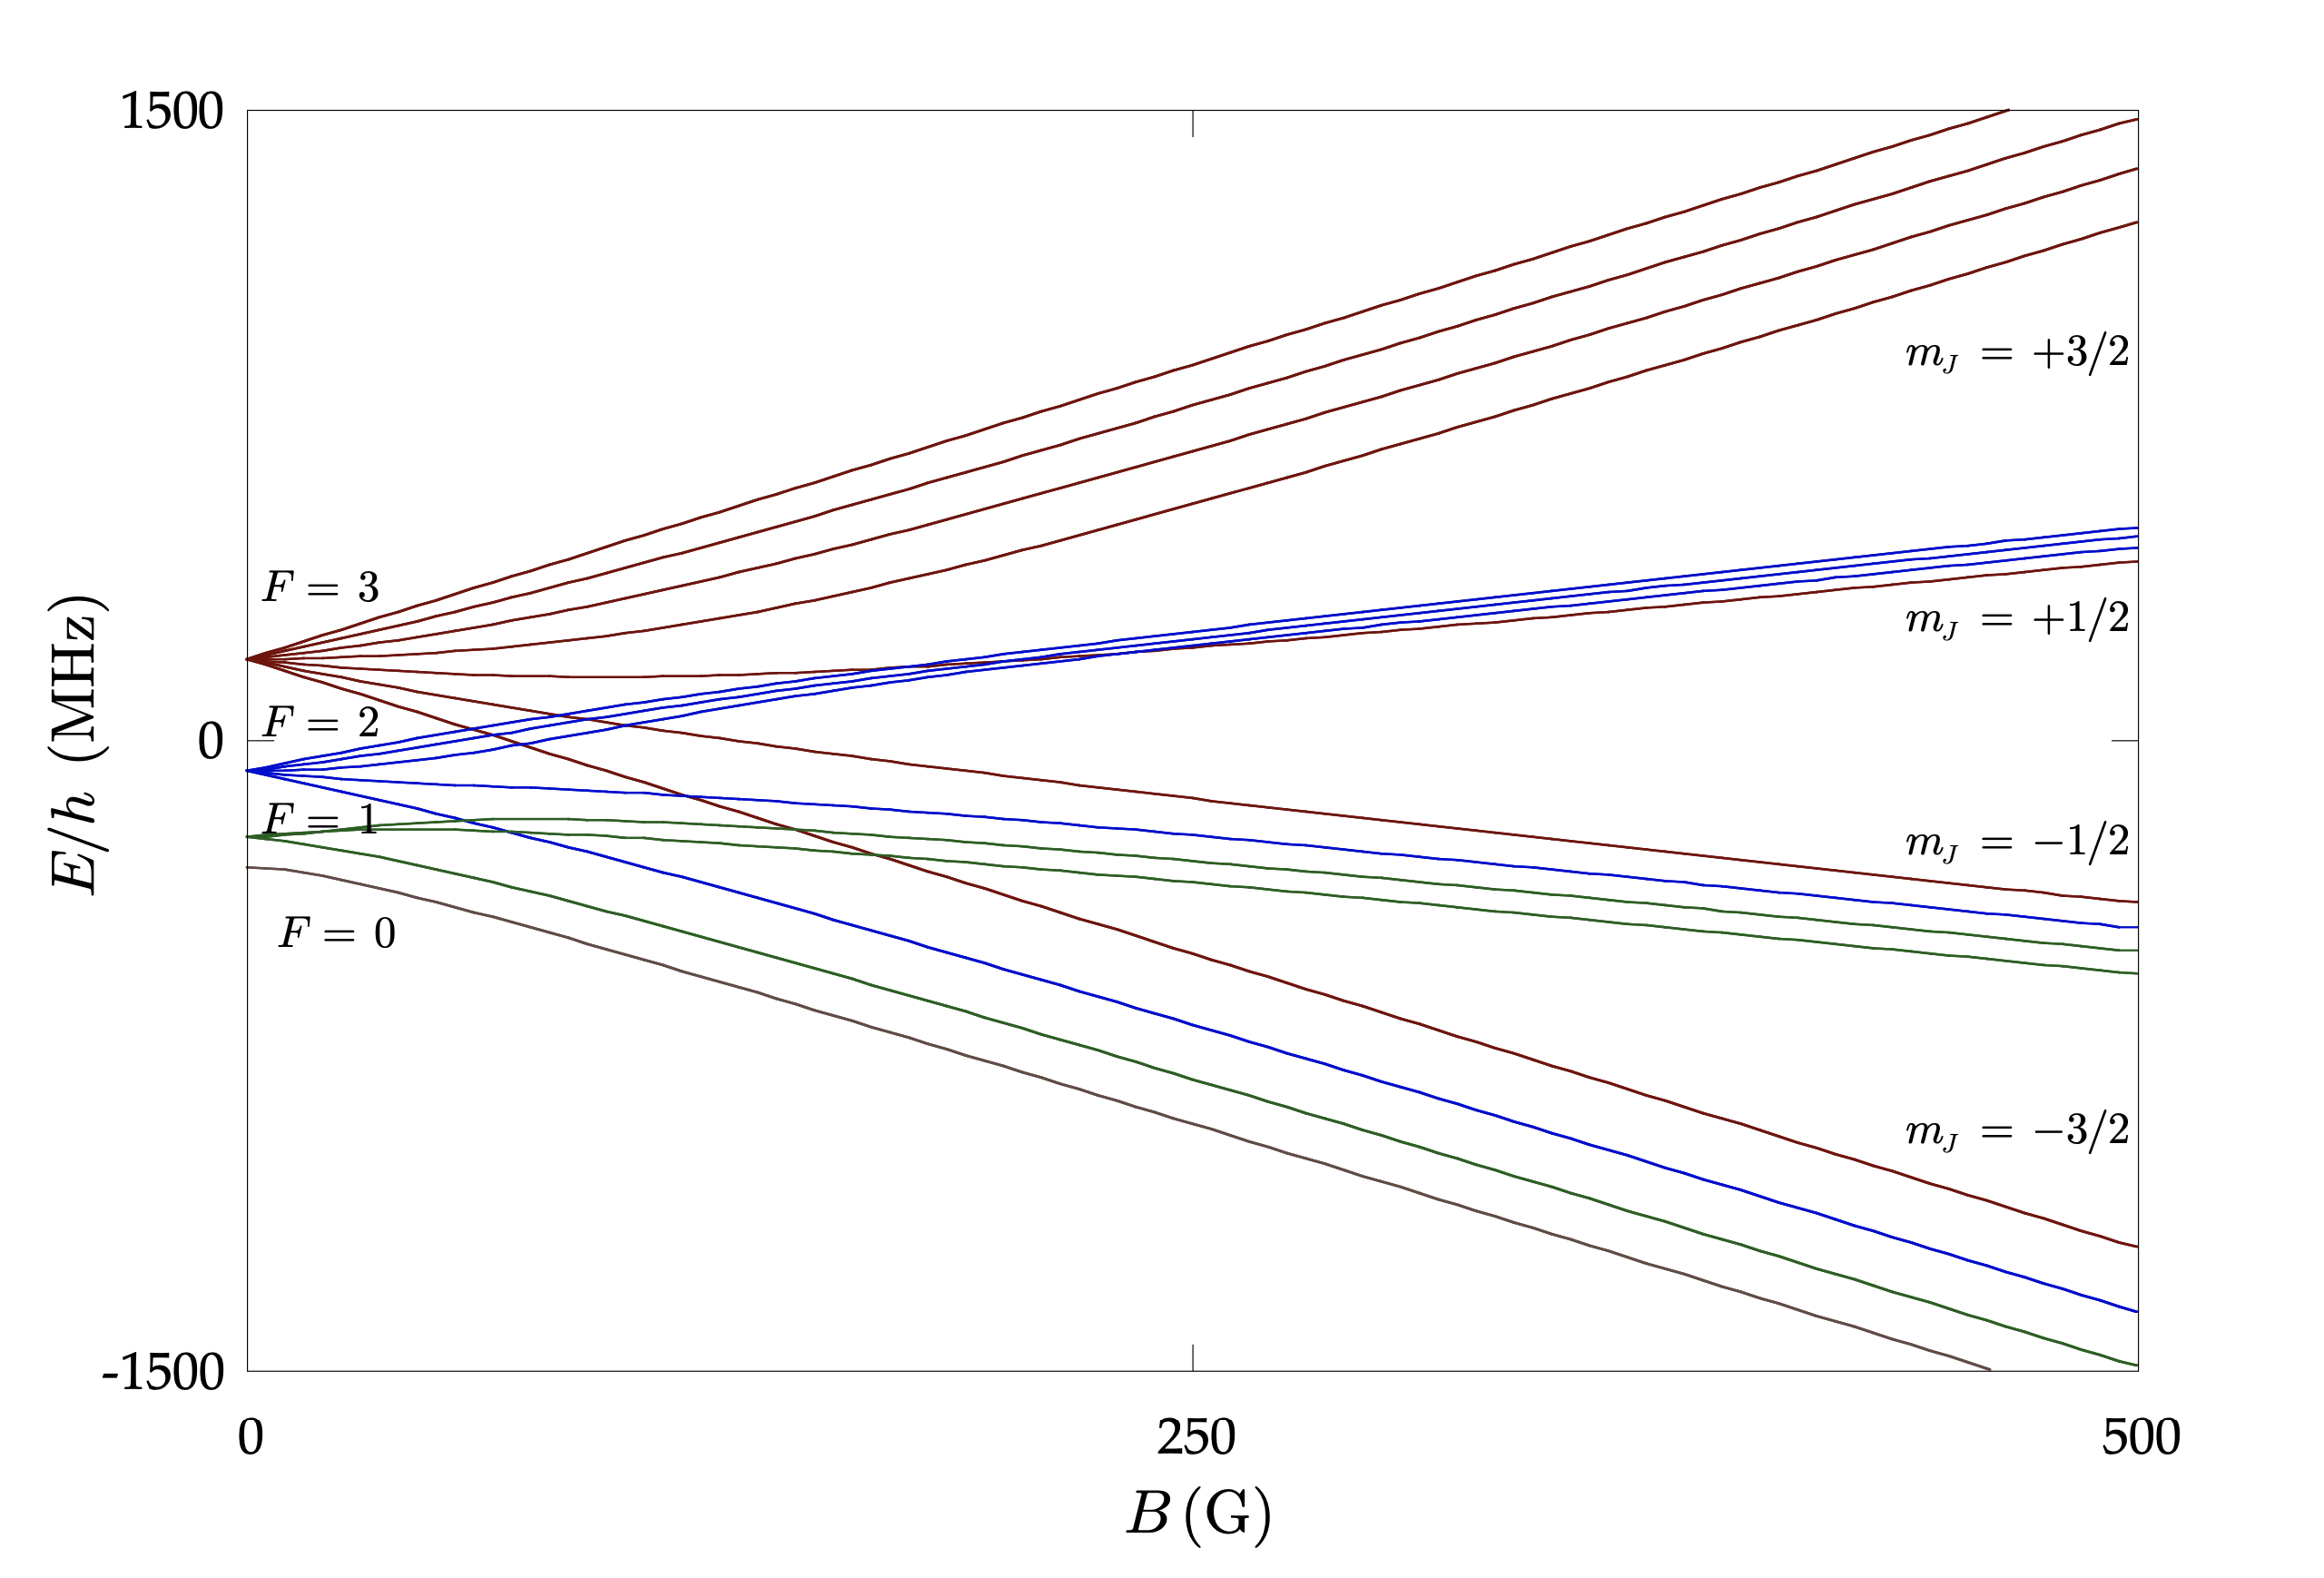
\epsfig{file=fig_zeeman.png, scale = .15}
\end{center}
\caption{The hyperfine structure of Rubidium-87 in an external magnetic field. \cite{steck} }
\end{figure}

Once the hyperfine levels are split, the atoms are exposed to two counter-propagating lasers with different polarizations of light that are red detuned, as shown in \textbf{1.4}. 

\begin{figure}[h!]
\begin{center}
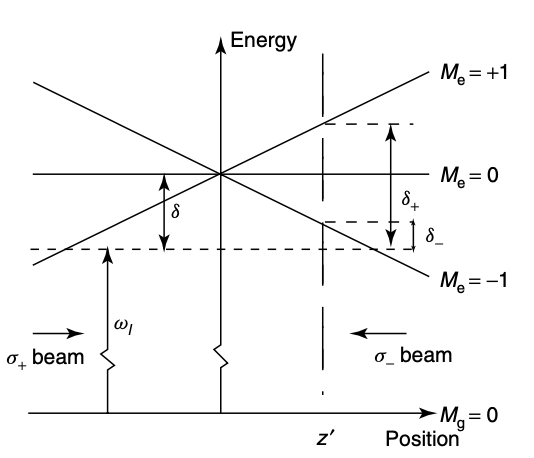
\epsfig{file=fig_MOT.png, scale = .8}
\end{center}
\caption{Visualization of the Zeeman splitting in a magneto-optical trap.   \cite{steck} }
\end{figure}

In a magneto-optical trap, one can imagine two different phenomena occurring. Atoms that are moving fast towards a laser, like in the case of optical molasses, see a light that is more on resonance, so they are more likely to be scattered. In addition, atoms that move away from the center of the trap experience Zeeman splitting. An atom in a position where $z'$ is greater feels a magnetic field that causes the transition where $\Delta M_F = -1$ to become more on resonance and therefore the atoms are more likely to experience a scattering force towards the negative $z'$ direction. When $z'$ is less, the transition where $\Delta M_F = -1$ is more on resonance and so the atom is more likely be scattered to the right by the positive circularly polarized light beam. Formalizing this idea,\cite{foot}

\begin{equation}
        \begin{aligned}[b]
    F_{MOT} &= F_{scatt}^{\sigma^+}(\omega - k\nu - (\omega_0 + \beta z)) - F_{scatt}^{\sigma^-}(\omega + k\nu - (\omega_0 -\beta z)) \\
    & \approx -2 \frac{\partial F}{\partial \omega} k \nu -2 \frac{\partial F}{\partial \omega} \beta z \\
    &= F_{damping} + F_{restoring}
        \end{aligned}
\label{eqn2.qo}
\end{equation}

Under these forces, the atoms undergo over-damped simple harmonic motion. A magneto-optical trap is typically the first step in cooling atoms and is the first step in the NASABEC machine. This machine uses both a two dimensional and three dimensional magneto-optical trap to cool the atoms via a laser. The 2D trap catches heated Rubidium atoms from the air, cooling them. From there atoms leak and are pushed up to the 3D magneto-optical trap which is tuned to be more effective at slowing already cooled atoms to about the Doppler limit, $100 \mu K $. From there, a phase of optical molasses allows for sub-Doppler cooling. The transition for this process in the NASABEC machine is $| F=2\rangle \rightarrow |F'=3\rangle$. Occasionally, while unlikely, atoms will be excited from the $| F=2\rangle$ state to the $| F'=2\rangle$ state and fall down to the $| F=1\rangle$ state. Atoms in the $| F=1\rangle$ state can not be properly cooled. For this reason, a repump beam on resonance with the $| F=1\rangle \rightarrow |F'=2\rangle$ transition is used to repopulate the atoms to the $|F=2\rangle$ state. Over time, the atoms will settle in the $|F=2\rangle$ state, where they can be effectively trapped and cooled. 
\newline

\subsection{Optical Pumping}

The next step in the cooling process is to get a method to trap the atoms without relying on a magneto-optical trap, which will only allow cooling towards the Doppler limit. For this process to be effective the sub-states of the atoms must be purified.

To understand the rules of optical pumping, one must understand the allowed energy level transitions, for which quantum mechanics explain\cite{introQM}. Due to conservation laws, the only transitions that are allowed are those for which $\Delta F = 0, \pm 1$ and $\Delta M_F = 0, \pm 1$. The energy levels for Rubidium-87 can be found as \textbf{Figure A.1} in \textbf{Appendix A}. The hyperfine splitting, the energy difference in the $M_F$ states, is determined by the Zeeman effect.

Hyperfine splitting effects on the required laser frequency are negligible. Controlling transitions for $\Delta F$ is easy as the energy levels vary significantly. The Ultra-Cold Atom Lab uses the $| F=2, M_F = 2\rangle$ state as the trappable state. To understand how the $M_F$ state is purified, a formalization of the polarization of light is helpful.
\newline

\subsubsection{Polarization of Light}
This section will review the concept of light polarization and introduce Jones Vectors. Recall that the polarization of light is described by the direction its electric field points over time. It is known, from the solutions to Maxwell's equations, that the electric field for light is described by 
\beq
\boldsymbol{E}(z,t) = (E_x\boldsymbol{\hat{x}} + E_y \boldsymbol{\hat{y}})e^{i(kz-wt)}
\eeq
\beq
\boldsymbol{E}(z,t) = (|E_x|e^{i\phi_x}\boldsymbol{\hat{x}} + |E_y| e^{i\phi_y}\boldsymbol{\hat{y}})e^{i(kz-wt)}
\eeq
where $k$ is the wave number. Factoring out the effective electric field,
\beq
\boldsymbol{E}(z,t) = E_{eff}(A\boldsymbol{\hat{x}} + B e^{i\delta}\boldsymbol{\hat{y}})e^{i(kz-wt)}
\eeq
where 
\beq
E_{eff} = \sqrt{|E_x|^2 + |E_y|^2}e^{i\phi_x}
\eeq
\beq
A = \frac{|E_x|}{\sqrt{|E_x|^2 + |E_y|^2}}
\eeq
\beq
B = \frac{|E_y|}{\sqrt{|E_x|^2 + |E_y|^2}}
\eeq
\beq
\delta = \phi_y - \phi_x
\eeq
This formalism is helpful as it can describe the proportion of the electric field in the $x$ and $y$ directions using $A$ and $B$. The angle $\delta$ describes the angle between the maximum $E_x$ and $E_y$ components. 

Jones Vectors use the following notation to describe how the electric field propagates:
\beq
\begin{bmatrix} 
A\\
Be^{i\delta}\\
\end{bmatrix} 
\eeq
Using this, the polarization of any plane wave field, which the laser light can be approximated to, can be described. For linearly polarized light, polarized at an angle $\alpha$ from the $x$ axis, the Jones Vector is 
\beq
\begin{bmatrix} 
cos\alpha\\
sin\alpha\\
\end{bmatrix} 
\eeq
For right, or positive, circularly polarized light the Jones Vector is
\beq
\frac{1}{\sqrt{2}}
\begin{bmatrix} 
1\\
-i\\
\end{bmatrix} 
\eeq
In this case, the angle between the maximum $E_x$ component and $E_y$ component differ by a factor of $\frac{\pi}{2}$ and the electric field rotates positively around the axis of propagation. 

A polarizer, a tool that changes the polarization of the light, can be represented as a $2x2$ matrix. A half-wave plate controls the orientation of linearly polarized light. Half-wave plates can be used in conjunction with a beam splitter, an object that lets linear polarized light aligned with its axis pass and reflects the component of light that is not. This is sometimes required because in reality half-wave plates are not perfectly effective. This combination can also split the beam in two paths, where the ratio of light transmitted and reflected can be controlled by changing the axis of linear polarization by turning a half-wave plate. A quarter-wave plate changes linearly polarized light into circularly polarized light and vice versa. The Jones Matrix for a half-wave plate is
\beq
\begin{bmatrix} 
cos2\theta & sin2\theta\\
sin2\theta & -cos2\theta\\
\end{bmatrix} 
\eeq
The Jones Matrix for a quarter-wave plate is
\beq
\begin{bmatrix} 
cos^2\theta +isin^2\theta & (1-i)sin\theta cos\theta \\
(1-i)sin\theta cos\theta & sin^2\theta + icos^2\theta\\
\end{bmatrix} 
\eeq
A quarter-wave plate works by slowing the electric field in one axis until the angle between the maximum $E_x$ and $E_y$ components differ by a factor of $\frac{\pi}{2}$. The magnitude of this phase difference depends on the thickness of the wave plate, $d$, and its refractive index along each axis, which is achieved in the way the crystal is cut. 
\beq
k_{slow}d - k_{fast} d = \frac{\pi}{2} +2\pi m
\eeq
For a half-wave plate
\beq
k_{slow}d - k_{fast} d = \pi +2\pi m
\eeq
where $m$ is any integer. When $m=0$, the wave plate is referred to as a zero order waveplate. A zero order wave plate tends to be more effective in practice. The Ultra-Cold Atom uses all of these optical tools to control the polarization and transmission of laser light as will be shown in \textbf{Chapter 3}.
\newline


\subsubsection{Optical Pumping of Rubidium-87}
\textbf{Figure 1.5} shows the allowed state transitions, where the transition the laser is on resonance with is the $| F=2\rangle \rightarrow |F'=3\rangle$ transition. 


\begin{figure}[h!]
\begin{center}
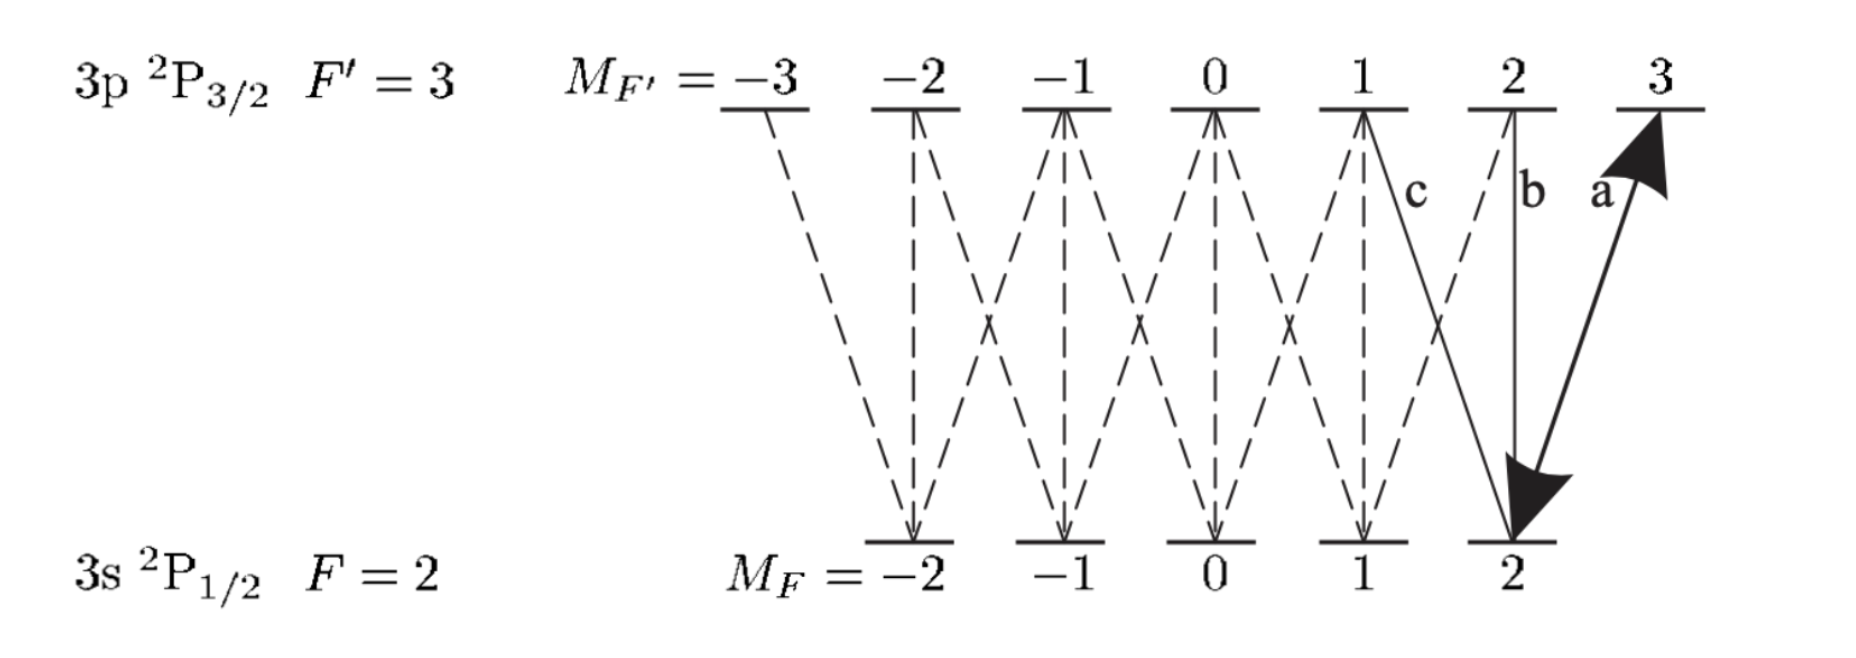
\epsfig{file=fig_allowed_transitions.png, scale = .5}
\end{center}
\caption{The allowed transitions between $| F=2\rangle \rightarrow |F'=3\rangle$. \cite{foot} }
\end{figure}

In addition, only positive circularly polarized light, $\sigma^+$, is used to pump the atoms. The axis of propagation is aligned with the applied external magnetic field so that the dipole moments of the atoms are aligned such that the atoms see positive circularly polarized light without a superposition of linearly polarized light or negative circularly polarized light. Doing this ensures that $\Delta M_F = 1$. Doing this, the atoms eventually begin to settle into the $M_F=2$ substate. With one scatter, the atoms either keep the same state, if $\Delta M_F = -1$ when they fall down to $F=2$, or increase their substate. Once in the $| F=2, M_F = 2\rangle$ state, atoms cycle between the $| F=2, M_F = 2\rangle$ and the $| F'=3, M'_F = 3\rangle$ states. Excessive scattering causes unnecessary heating of the atoms. This process is very fast so the laser must be detuned to not heat the sample. This is explored in \textbf{Chapter 2}. \textbf{Figure 1.6} shows the relative probabilities when driving transitions from the $| F=2\rangle$ state with $\sigma^+$ light.

\begin{figure}[h!]
\begin{center}
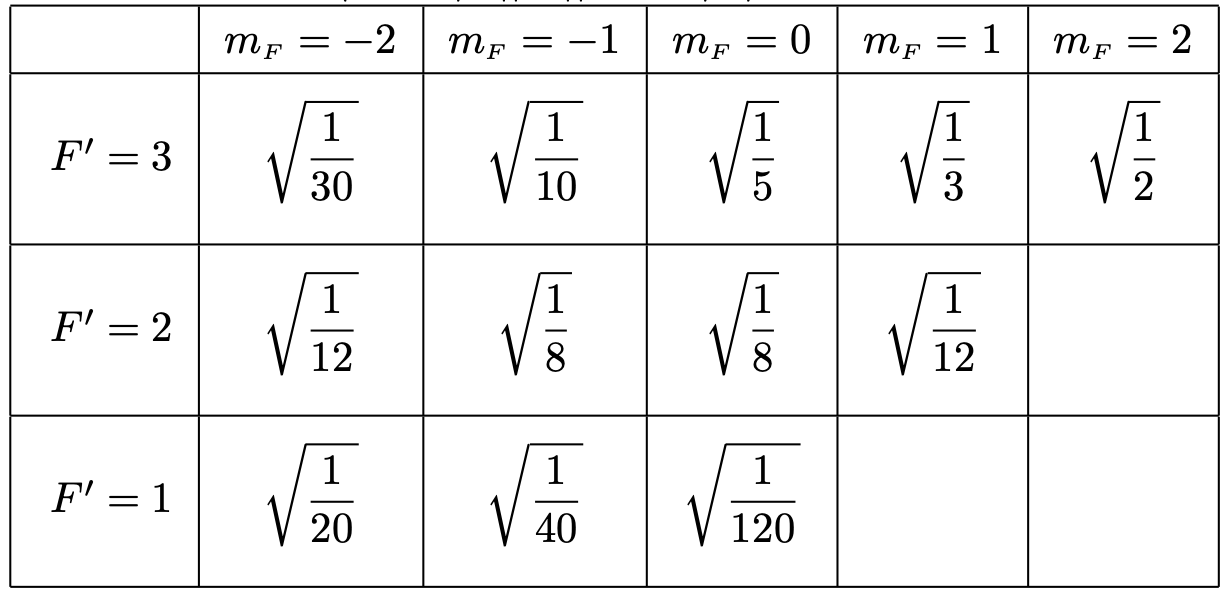
\epsfig{file=fig_trans_table.png, scale = .5}
\end{center}
\caption{The relative probabilities for transitions from $F=2$ with $\sigma^+$ light. \cite{steck} }
\end{figure}

Squaring and doubling these probabilities gives the absolute probabilities between transitions. 
\begin{figure}[h!]
\begin{center}
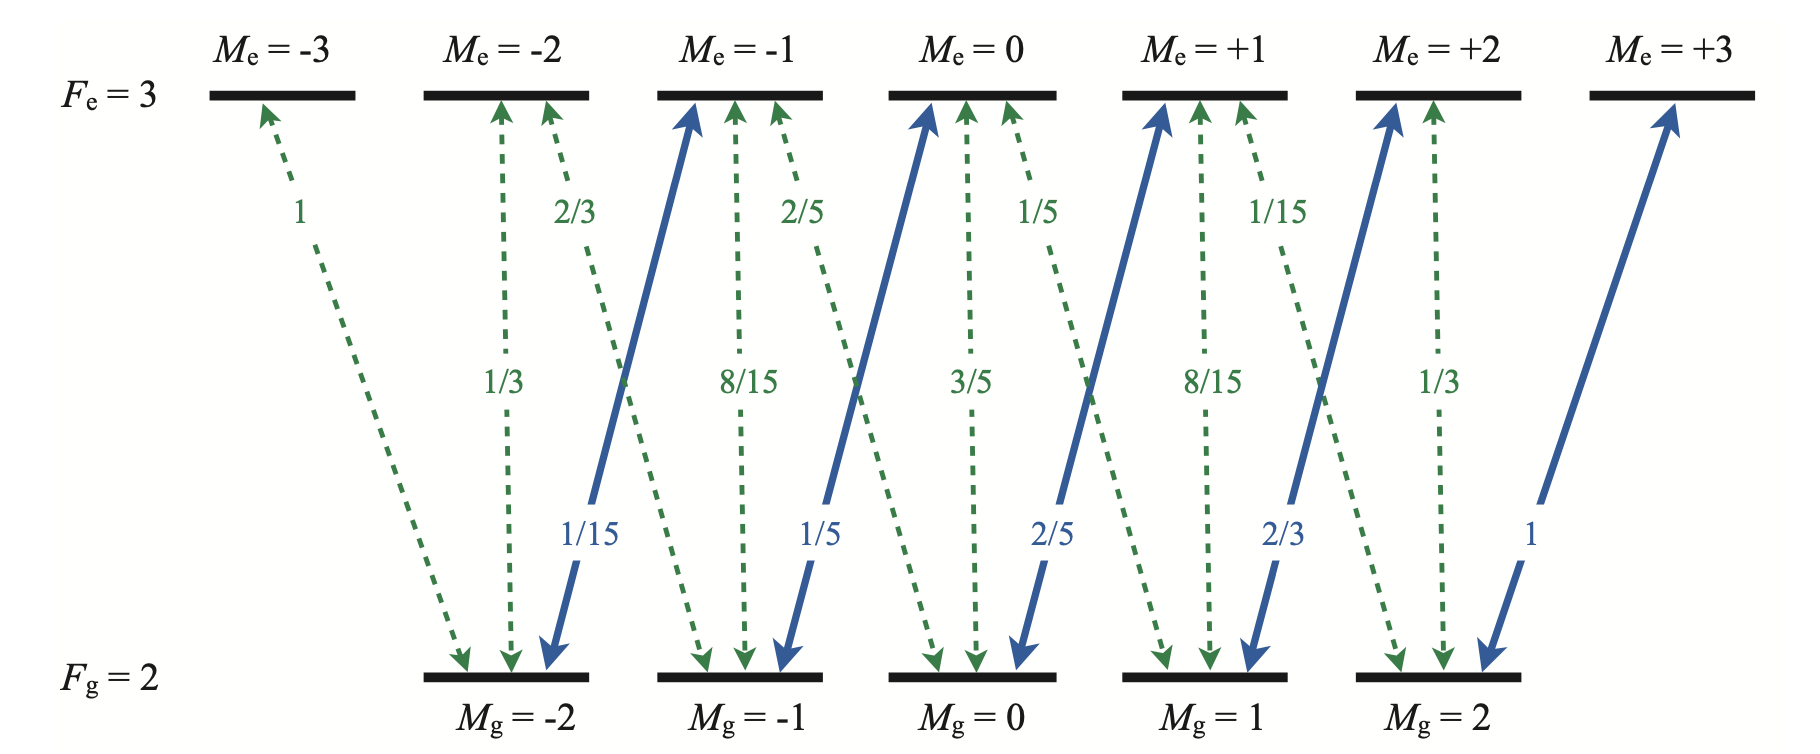
\epsfig{file=fig_rel_probabilities.png, scale = .5}
\end{center}
\caption{The relative probabilities for transitions between $F=2$ and $F'=3$ with $\sigma^+$ light. \cite{Atoneche} }
\end{figure}

Once most of the atoms are purified into the $| F=2, M_F = 2\rangle$ state, they can be effectively trapped by a magnetic trap tailored to capture atoms with the corresponding magnetic dipole. Originally, had the magnetic trap been turned on without optical pumping, states where $M_F$ is negative would be repulsed. Atoms with $M_F=0$ would not feel any force and succumb to gravity. Atoms where $M_F=1$ would not experience as strong of a trapping force and therefore could leak out of the trap with their sufficiently large kinetic energies. Optical pumping purifies the atoms to ensure that they are effectively trapped. 
%%could talk about leakage, probably uneccessary tho

\subsection{Evaporative Cooling}
The final step in Bose-Einstein Condensation formation is evaporative cooling. Evaporative cooling works by removing the atoms with the highest thermal energy to decrease the temperature of the atom cloud by multiple orders of magnitude. This process requires a mechanism to biasedly remove the hottest atoms and a sufficiently high energy transfer rate to reestablish thermal equilibrium. This must be done without decreasing the density of the atoms so that the phase space density increases until the atoms form a Bose-Einstein Condensate. This process is similar the a way a hot cup of coffee cools off, where the hottest atoms evaporate off. 

At this stage, the temperature distribution of the gas can be well approximated by a Boltzmann distribution.
\beq
N(E) = N_0e^{-E/k_bT_1}
\eeq 
where $N(E)$ is the number of atoms with an energy $E$ and $T_1$ is the characteristic temperature. From this distribution, a cutoff energy is chosen and atoms with energies higher than that energy are removed from the trap in a mechanism discussed later. This is referred to as using an RF-knife (radio-frequency). From there, thermal equilibrium is reestablished and a lower cutoff energy is chosen. This process is repeated until the cloud reaches a temperature on the order of about $100nK$ and a Bose-Einstein Condensate is formed. In practice, the process is more continuous as thermal equilibrium is reached sufficiently fast. 

\begin{figure}[h!]
\begin{center}
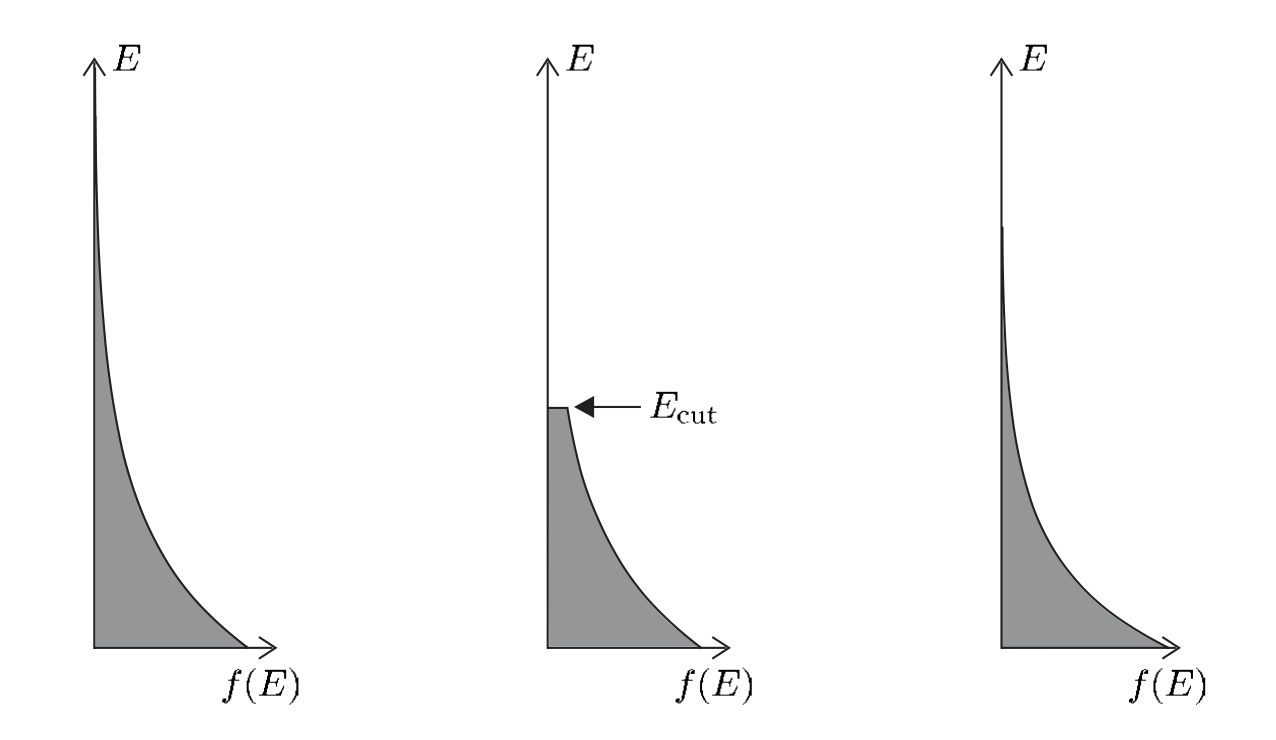
\epsfig{file=fig_e_cutoff.png, scale = .5}
\end{center}
\caption{A visualization of the evaporative cooling process. $f(E)$ is the energy density defined by a Boltzmann distribution. \cite{foot} }
\end{figure}

This mechanism uses what is known as an RF-knife. For this to work, and to keep the phase density of the atoms high, the strength of the magnetic trap is greatly increased. From there, the quadratic Zeeman effect is no longer negligible. The substates of the $|F=2\rangle$ state spread more dramatically as the atoms leave the from the center of the trap. Atoms with higher kinetic energies reach the further edges of the trap as only they have enough energy to overcome the stronger magnetic potential energy. When an atom is farther from the center of the trap its $M_F$ states become more separated as shown in \textbf{Figure 1.9}. 
\begin{figure}[h!]
\begin{center}
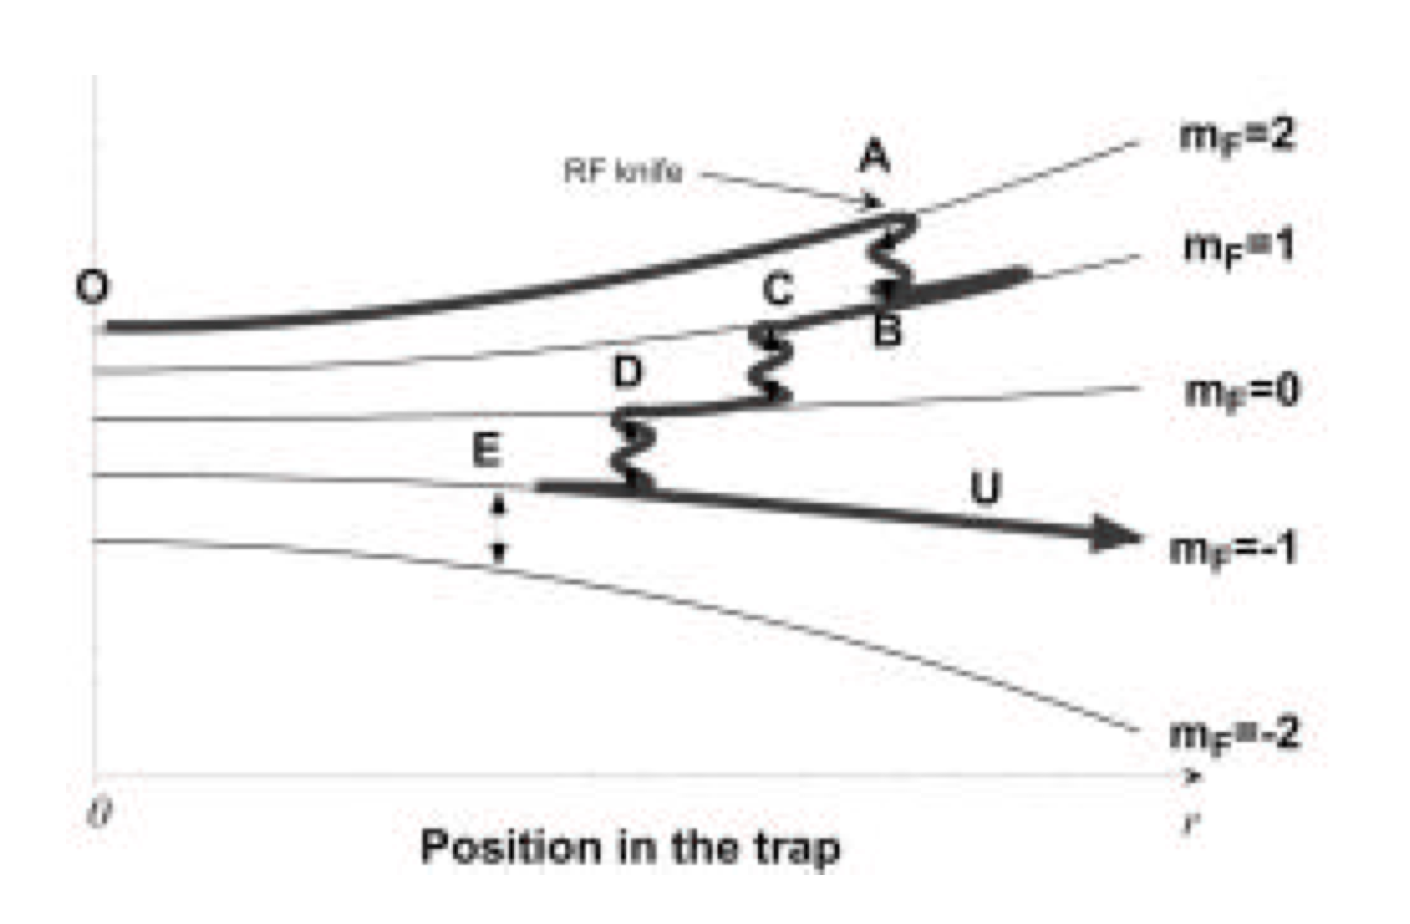
\epsfig{file=fig_quad_zeeman.png, scale = .3}
\end{center}
\caption{A visualization an atom above $E_{cut}$ being removed from the trap. \cite{bouyer} }
\end{figure}

The atoms are exposed to radio frequency light that is tuned such that it is only on resonance for an atoms whose $M_F$ states are sufficiently separated like the difference between \textbf{A} and \textbf{B} in \textbf{Figure 1.9}. At that point, the atom can be excited into lower sub-levels, as the atoms move around the trap, until the magnetic trap forces it out of the trap when $M_F=-1$. The result is not always as shown. An atoms could be re-excited back into a higher energy state should it be the correct distance from the center of the trap. Nonetheless, atoms with sufficiently high energies will eventually be removed from the trap. This final step is repeated until a Bose-Einstein Condensate is formed. 
\chapter{Computational Simulation of Optical Pumping}
This section explores optical pumping through a simulation. The substates of the $|F=2\rangle$ state are modelled as they undergo scattering. This simulation was done in Python3, using the numpy, matplotlib, and sklearn libraries for analysis, regressions, and creating figures. Due to the efficiency of the repump laser and the small amount of leakage, the $|F=1\rangle$ state is not considered in this simulation. The simulation explores the trade off between the final purity of the optical pumping process and the amount of photon scattering, which heats the atom cloud. The number of scatters per atom, on average, required to purify the atoms is a central theme of the simulation. As the optical pumping process happens very fast, faster than the time the mechanical shutter can be turned on and off, the final goal of the simulation is to relate the number scatters required per atom to a required detuning rate to both purify a sufficient percent of the atoms and not overheat the sample. This relation happens from the process described in \textbf{Equation 1.16}
\begin{align*}
R_{scatt} = \frac{\Gamma}{2} \frac{\frac{I}{I_{sat}}}{1 + \frac{I}{I_{sat}} + 4 \left( \frac{\delta}{\Gamma}\right)^2 } \tag{1.16}
\end{align*}
Where $\delta$ is the frequency detuning of our laser. 

\section{Building a Model}

The simulation modeled the population of the ground states, the states of interest, by uniformly populating a 5 element list with integers representing the number of Rubidium atoms in the atom cloud that are in a corresponding $M_F$ substate. This uniform distribution is expected at this stage. From there, a function randomly chooses one of these atoms to excite. The atom chosen is random and therefore choosing an atom from a specific $M_F$ substate depends on the relative population of atoms in a particular $M_F$ substate. From there, the atom obeys selection rules. Since the atom is exposed to positive circularly polarized light along its magnetic dipole moment, it will absorb the angular momentum of the photon and will increase its substate, $|F'=3, M'_F = M_F + 1 \rangle$. Once excited, the atom falls back to $F=2$, choosing its $M_F$ substate based off the relative probabilities described by quantum mechanics in \textbf{Figure 1.7}. This process is repeated, keeping track of the atom cloud states and the number of photon scatters. This model is effective in many ways. It can be used to show the relative population of atom substates over time. The relation is between photons scattered and the proportion of the atoms in the trappable $M_F=2$ substate. From there, as heating increases with the number of photons scattered, an intuitive relation is shown between heating and the number of trappable atoms. In addition, the number of scatters required per atom is easily related to the required intensity and frequency detuning through \textbf{Equation 1.16}.

The model is first run on a theoretical cloud of 100 Rubidium atoms as shown in \textbf{Figure 2.1}.



\begin{figure}[h!]
\begin{center}
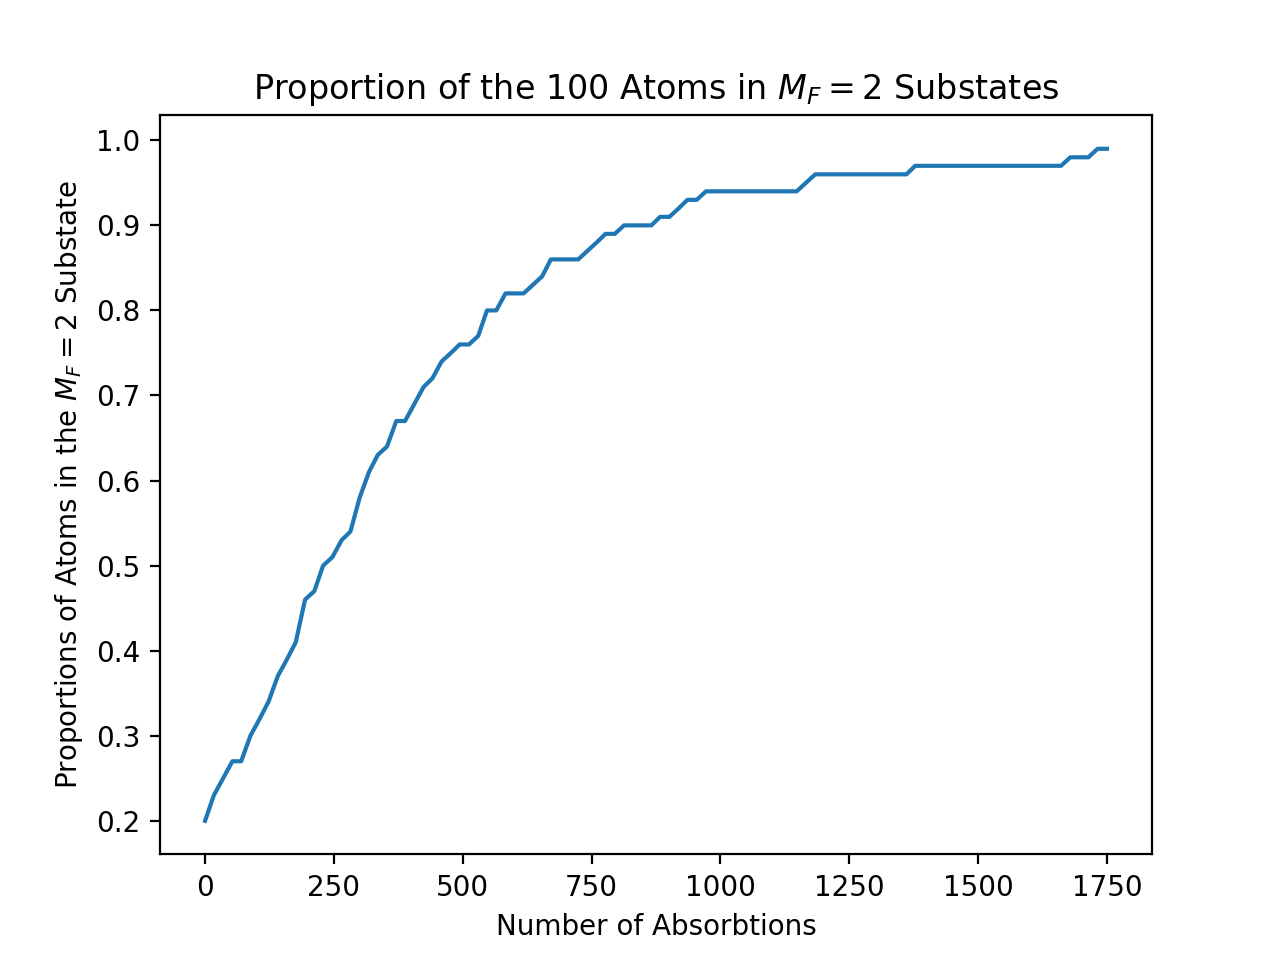
\epsfig{file=fig_prop_atoms_lin.png, scale = .75}
\end{center}
\caption{A visualization of the simulation on a cloud of 100 Rubidium atoms. }
\end{figure}

This figure confirms intuitions on the optical pumping process. Once trapped, atoms do not change their $M_F$ substate, even if they are excited. This is because they will cycle between the $|F=2, M_F=2\rangle$ and $|F'=3, M'_F=3\rangle$ states. It is also clear that getting more atoms in the desired state requires more and more photon scattering as the purity gets high. This is because already trappable atoms start to become scattered more often. This causes unnecessary heating. This can be more accurately viewed in \textbf{Figure 2.2}.

\begin{figure}[h!]
\begin{center}
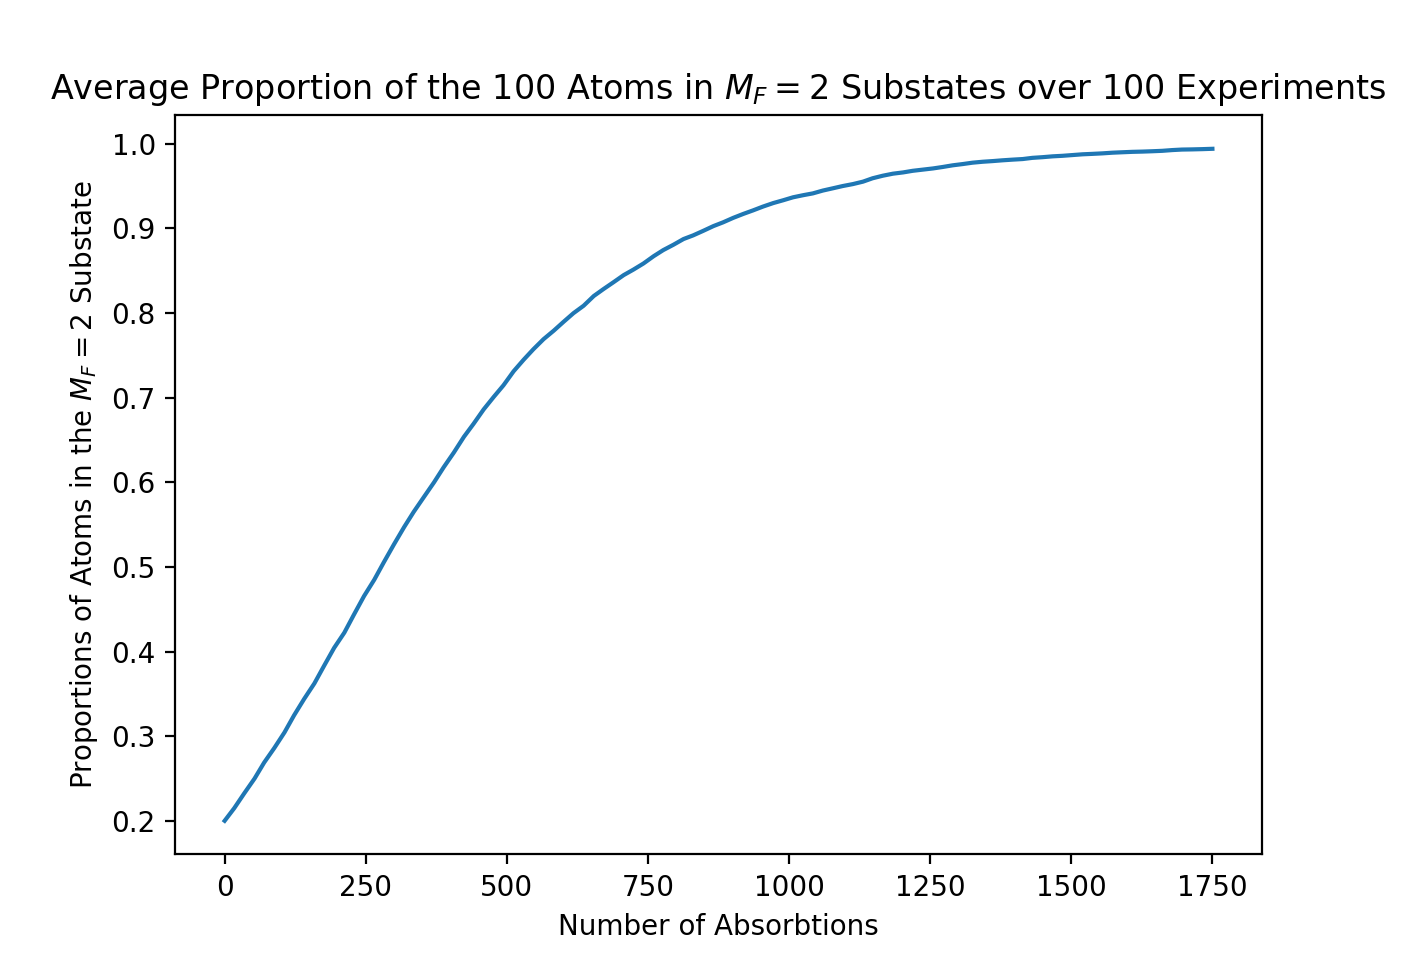
\epsfig{file=fig_avg_lin.png, scale = .75}
\end{center}
\caption{A visualization of the simulation run on a cloud of 100 Rubidium atoms 100 times and averaged. }
\end{figure}

This illustrates the cost-benefit of more photon scattering. At a certain point, achieving a certain purity is no longer desirable as it requires a large amount of scattering and heating of the system. On the NASABEC machine, there are other steps with much higher losses of atoms. While the optical pumping process should be an efficient process, other steps could be optimized if the number of atoms in the Bose-Einstein Condensate is not sufficient. For that reason, the difference between, say, a $95\%$ purity and a $99\%$ purity, is mostly negligible. 
\newline

\section{Scaling the Model}

While this initial model is informative, it cannot be run on a cloud of millions of atoms, like in the lab. The computational requirements are simple too large and could not be completed in time. Nonetheless, the model can be changed to gain intuition on how many photon scatters are required as the atom cloud grows. If a relation can be found between the number of photon scatters and the number of atoms in the purified state, then this relation can be applied to atom clouds with millions of Rubidium atoms. 

To do this, the simulation models how many photon scatters are required to get to a given purity level. The different purity levels explored are $80\%$, $90\%$, $95\%$, and $99\%$. $50$ different atom cloud sizes are explored with each of these purity levels. The atom cloud sizes are linearly distributed from $100$ to $50000$. The simulation takes note of how many photon scatters were required to get each atom cloud to the different purity level. The results for these purity levels are shown below in \textbf{Figure 2.3}.

\begin{figure}[h!]
\begin{center}
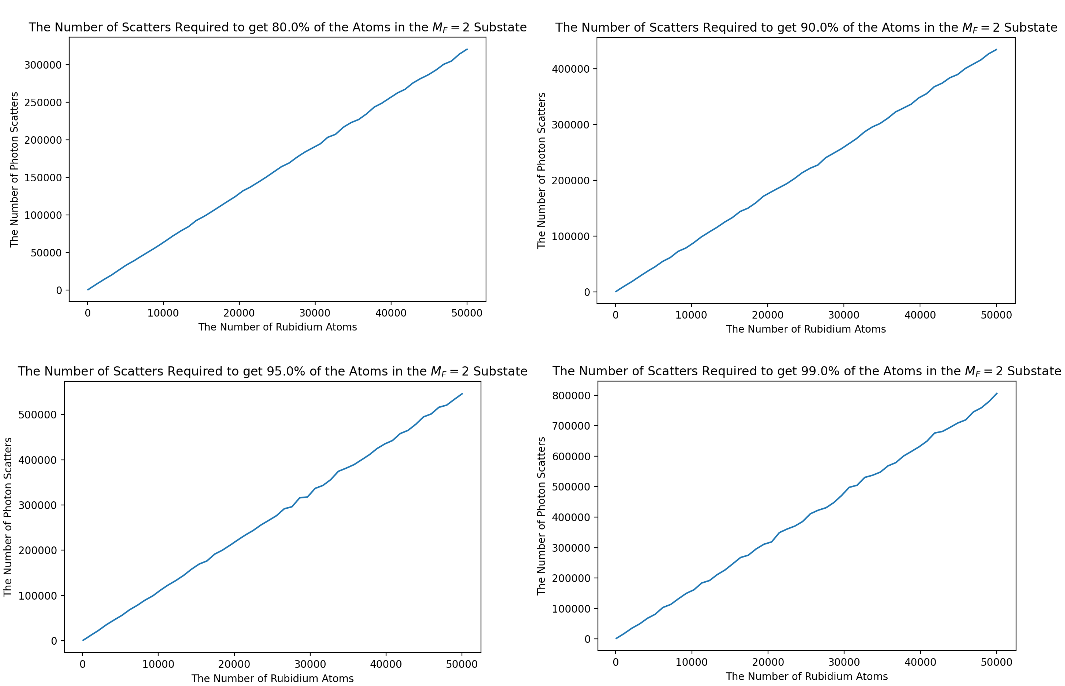
\epsfig{file=fig_many_scatters.png, scale = .45}
\end{center}
\caption{Visualizations of the amount of photon scatters required to trap different percentages of the Rubidium atoms. }
\end{figure}

These graphs show that getting a higher purity level for a given number of atoms requires significantly more scattering and heating. It is also clear from these graphs that the relationship between the number of photon scatters required to purify the atoms and the number of initial atom is linear. This leads to the conclusion that the number of photon scatters required per atom is independent of the number of atoms. This makes sense as, on average, any individual atom has an equal probability of being in any state and the number of scatters required to give the atom a particular probability of being in the trappable state is independent of the amount of Rubidium atoms. This conclusion also makes it possible to model how many scatters are required to purify an atom cloud with millions of atoms. The next step is to determine how many photon scatters is required per atom to get a given purity level. To do this, each of these plots is linearly regressed using a least-squares method. The estimated slope of this regression is the number of photon scatters required per Rubidium atom at the given desired purity level. These regressions are shown below in \textbf{Figure 2.4}.

\begin{figure}[h!]
\begin{center}
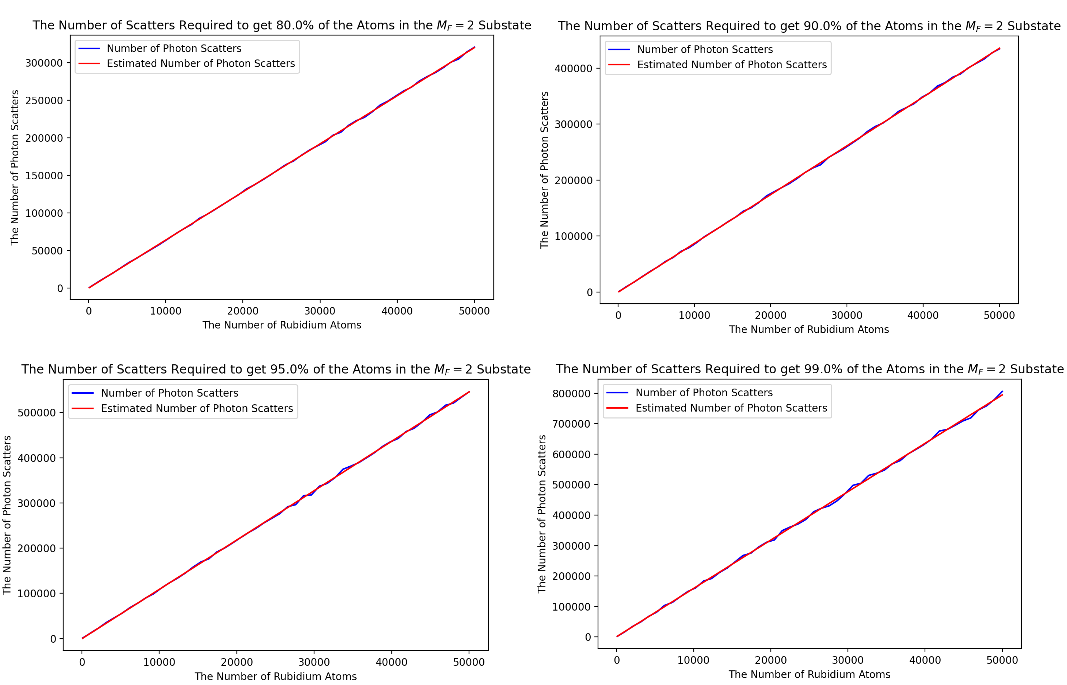
\epsfig{file=fig_many_scatters_reg.png, scale = .45}
\end{center}
\caption{Visualizations of the amount of photon scatters required to trap different percentages of the Rubidium atoms with a least-squares linear regression. }
\end{figure}

For each of these regressions, the coefficient of determination was greater than $99.9\%$, which agrees with the interpretation that the required photon scatters per atom is independent of the number of atoms. The calculated required photons scatterings for each of these experiments is shown in \textbf{Table 1}. 
\begin{table}[h]
\begin{center}
\begin{tabular}{|l|l|r|l|}
\hline
Percent of Atom in the $M_F=2$ State & Photon Scatters per RB Atom\\
\hline
80 & 6.41\\
\hline
90 & 8.72\\
\hline
95 & 10.92 \\
\hline
99 & 15.88 \\
\hline
\end{tabular}
\caption{The amount of scatters required per atom grows as the desired number of atoms in the $M_F=2$ trappable states grows.}
\end{center}
\end{table}

This gives some very accurate results for these purity levels. The amount of scatters per atom grows at an increasing rate. These numbers provide a good opportunity to make a decision of the desired purity levels. While the jump between $90\%$ and $95\%$ purity only requires a $25\%$ increase in the number of scatters, the jump between $95\%$ and $99\%$ requires a $45\%$ increase in the number of scatters. This significantly heats the sample for only $4\%$ more of the original atoms. For that reason, it will be decided that the purity level should be $95\%$. If that sounds low, recall that on other steps of the cooling process, much higher proportions of atoms are lost. Optimizing these steps would be significantly more beneficial to increasing the atom count of the Bose-Einstein Condensate. If that sounds high, it is worth noting that the optical pumping process is typically an efficient step in the process of making a Bose-Einstein Condensate. 

To further study the relation between the number of scatters required for a given purity, one more simulation was performed. This simulation explored more desired purities from $80\%$ to $99\%$. As the previous simulations took hours to run, the atom cloud size had to be greatly reduced. The atom cloud sizes studied for this experiment ranged from $1000$ to $5000$ atoms. Nonetheless, the same general trend can be extracted: the amount of photon scattering per atom grows as the desired purity level grows. 

\begin{figure}[h!]
\begin{center}
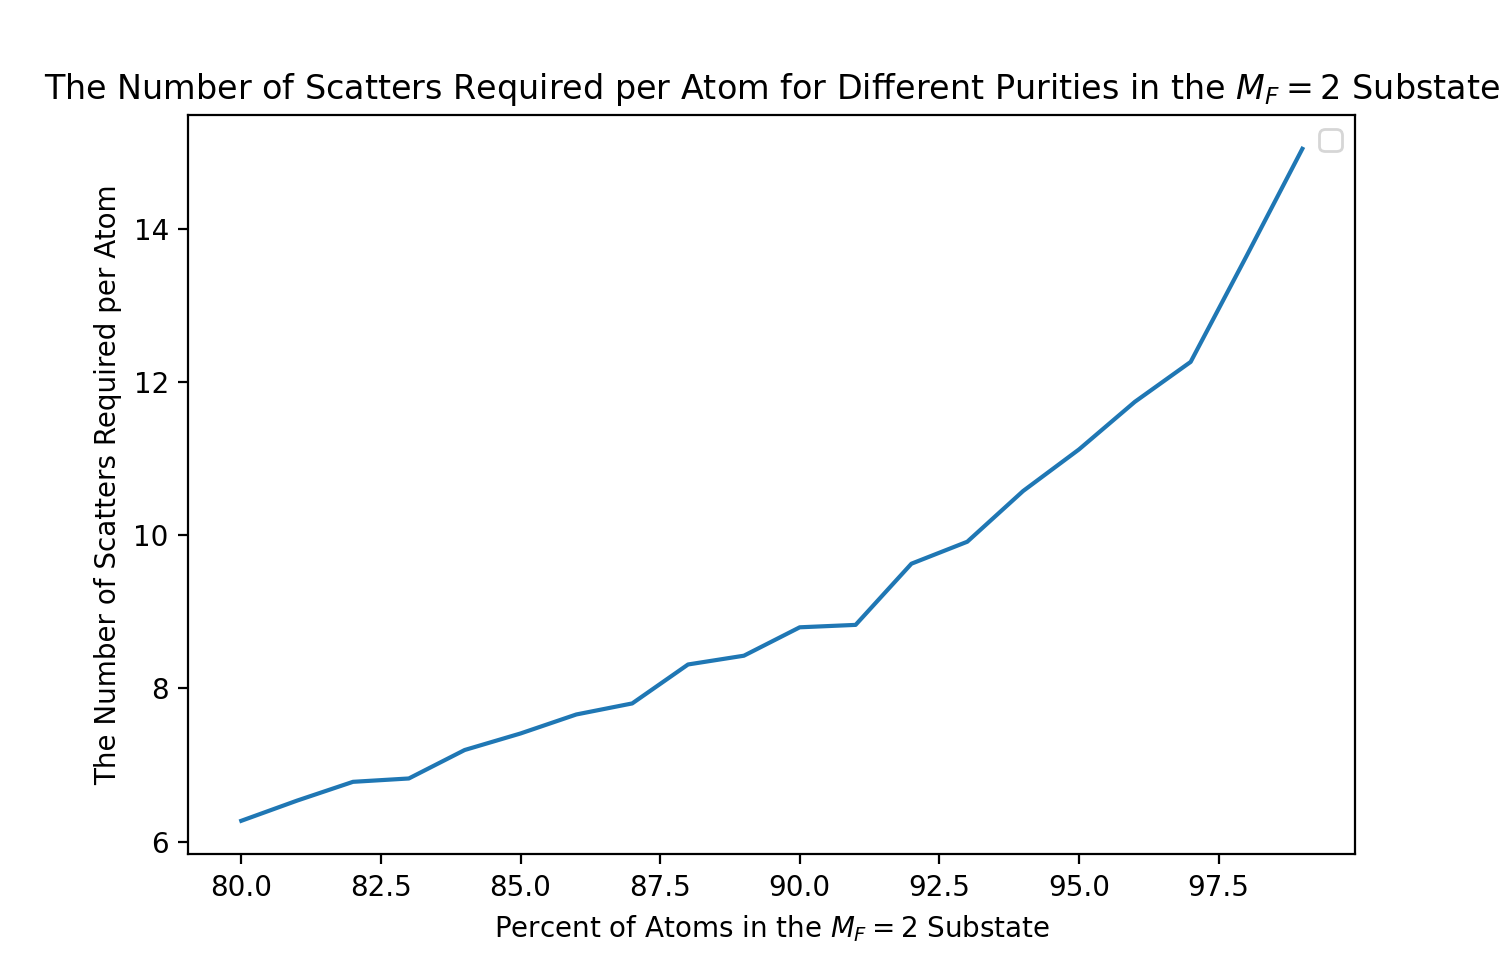
\epsfig{file=fig_scatt_purity.png, scale = .65}
\end{center}
\caption{The amount of scatters required per atom grows seemingly exponentially as the desired number of atoms in the $M_F=2$ trappable states grows. }
\end{figure}

The trade-off of the optical pumping process could be viewed in a different way. A higher purity, which results in more heating, requires more atoms to be lost in the evaporative cooling stage to form a Bose-Einstein Condensate. On the other hand, a lower purity does result in less heating but leaves less atoms to form the Bose-Einstein Condensate. As the final goal is to have the most atoms in our Bose-Einstein Condensate, there is a 'sweet-spot' here to be reached. 
\newline

\section{Calculating a Detuning Frequency}
As stated previously, the NASABEC machine will initially seek an optical pumping efficiency of $95\%$. To do this, each atom must, on average, be scattered by $10.92$ photons. \textbf{Equation 1.16}, which describes the scattering rate per atom at a given intensity and frequency detuning, can be used to calculate the parameters for which our laser must be set. Recall that this process typically happens very fast, faster than the mechanical shutter can open and close to allow the process to happen. Though the intensity could be changed in the lab, a fixed power will be assumed of about $4.75 mW$ leaving the optical fiber cable, as currently set up. Should this be changed, the calculation for the frequency detuning remains simple, knowing that each atom must scatter $10.92$ photons on average. In addition, another purity level can be chosen, and the calculations remain simple. Still, it is recommended to choose a purity level given in \textbf{Table 1} as these values were averaged over a large range of atom cloud sizes. 

\textbf{Equation 1.16} can be related to the number of scatters per atom by multiplying by the time the laser is shone on the atoms, $t_s$
\beq
10.9 = R_{scatt} t_s
\eeq
Substituting in \textbf{Equation 1.16} and solving:

\begin{equation}
        \begin{aligned}[b]
            10.9 &= R_{scatt} t_s\\
            10.9 &=  \frac{\Gamma}{2} \frac{\frac{I}{I_{sat}}}{1 + \frac{I}{I_{sat}} + 4 \left( \frac{\delta}{\Gamma}\right)^2 }t_s\\
            \frac{\delta}{\Gamma} &= \pm \sqrt{\frac{\Gamma\frac{I}{I_{sat}}t_s}{10.9*8} - \frac{1}{4} - \frac{1}{4}\frac{I}{I_{sat}}}
        \end{aligned}
\label{eqn2.qo}
\end{equation}
\beq
\delta = \delta(I, t_s) = \pm \sqrt{\frac{\Gamma\frac{I}{I_{sat}}t_s}{10.9*8} - \frac{1}{4} - \frac{1}{4}\frac{I}{I_{sat}}}\ \Gamma
\eeq
The two solutions mean that the laser can be red or blue detuned and the result will be the same. In this case, for driving the $|F=2\rangle \rightarrow |F'=3\rangle$ transition with $\sigma^+$ light, the saturation intensity is $I_{sat} = 1.669 mWcm^{-2}$ and the natural linewidth is $\Gamma = 38.11 * 10^6Hz$. The time the atoms will be exposed to this light is assumed to be $1.5$ milliseconds. 

To calculate the detuning frequency, the intensity of the light at the atoms must be calculated. The power of the linearly polarized light coming out of the optical fiber cable is $4.75 mW$. The efficiency of a quarter-wave plate, to make the light positive circularly polarized was measured to be $90\%$. As there is no culminating lens attached to the end of the optical fiber, this beam spreads significantly. To calculate the intensity that the atoms see, which is $15.5cm$ away from the optical fiber, two different distances and beam diameters were measured. It was assumed that the beam spread in a cone-like shape over this short distance. The intensity of the light at the atom was calculated to be about $1.669 mWcm^{-2}$. Using this intensity, the necessary frequency detuning can be calculated. 

\beq
\delta(I = 1.669 mWcm^{-2}, t_s = 1.5ms) =\pm 6.9\Gamma = \pm260 MHz
\eeq

The Doppler effect is neglected for this detuning as, on average, its result is zero. As the lasers are typically red detuned for optical pumping, the laser NASABEC machine should be red detuned $260 MHz$ to reach a $95\%$ purity of atoms in the $M_F=2$ trappable substate with our current laser parameters. This result is in agreement with another lab that uses a similar setup and has a frequency detuning of about $230 MHz$. Finally, it is worth noting that this model does not include the fact that the intensity of the laser could decrease across the atom cloud because the number of atoms is relatively small, so this effect is negligible. 

The code used in this section can be found in the \textbf{Appendix}. The main application of this program is to get an estimated required number of photon scatters per atom for a desired purity. After this value is calculated, \textbf{Equation 2.3} describes the relationship between the frequency detuning, laser intensity at the atoms, and the time the laser is to be pumping the atoms. Reiterating, should any of the laser parameters require changing (intensity, frequency detuning, or time pumping) this can easily done through \textbf{Equation 2.3}. 

%% in the other 
 % Use the same command to add more chapters or sections
\chapter{Experimental Approach and Procedure towards Optical Pumping} 
This section explains the setup and approach toward realizing optical pumping on the NASABEC machine. The main apparatus is ColdQuanta's RuBECi 2D+ and 3D MOT Chamber system. This section does not discuss the equipment setup for the 2D and 3D magneto-optical trap, repump beam, transfer coils, or ColdQuanta's Quadrupole Coil Assembly. More information on this equipment and the laser cooling steps can be found in previous alumni theses\cite{sshea}\cite{mcwik}\cite{dpaseltiner}.
\newline

\section{Building an Optical Pathway to the NASABEC}
The first step in creating an optical pumping process is getting light to the RuBECi apparatus. The table that houses the laser and laser amplifier is about 1.5 meters away from the table where the RuBECi machine is mounted. In addition, there was no laser power designated for optical pumping. The setup for this section is shown in \textbf{Figure 3.1} and \textbf{Figure 3.2}. 

\begin{figure}[h!]
\begin{center}
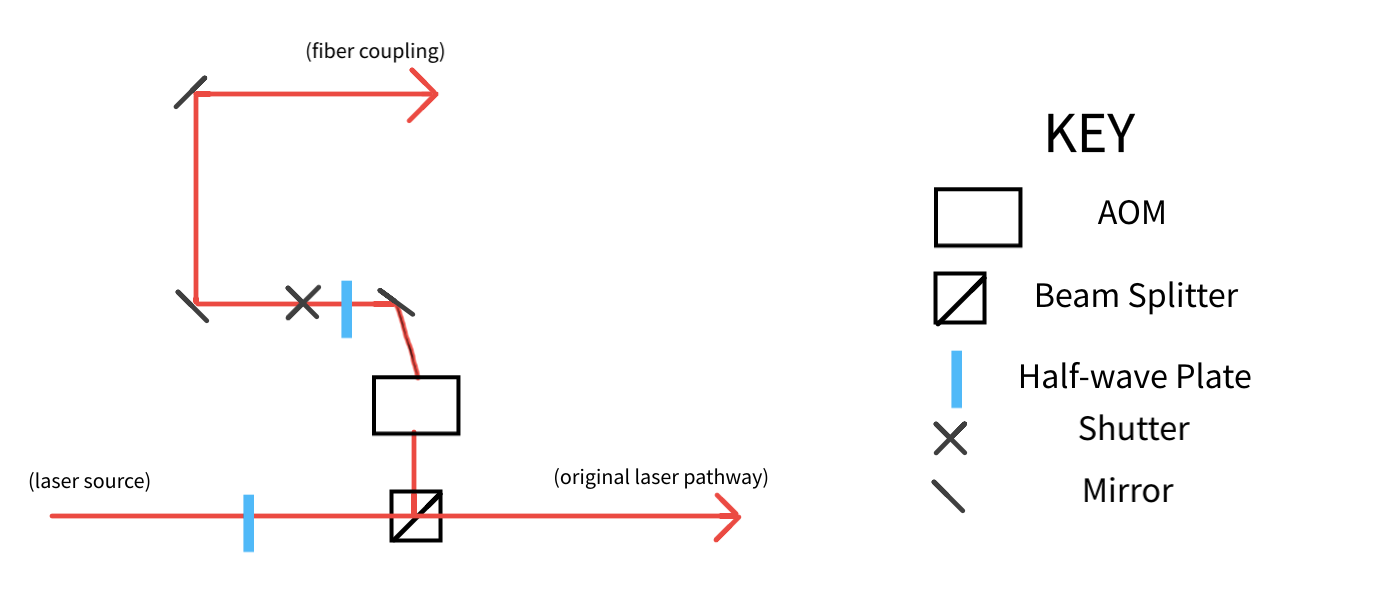
\epsfig{file=fig_setup_drawing.png, scale = .6}
\end{center}
\caption{A schematic diagram of the optical pathway for to get light to the RuBECi machine. }
\end{figure}

\begin{figure}[h!]
\begin{center}
\epsfig{file=fig_first_table.jpg, scale = .1195}
\end{center}
\caption{A picture of the optical pathway for to get light to the RuBECi machine. }
\end{figure}

To create this optical pathway, some of the laser's power was extracted with a half-wave plate and beam splitter. These devices were placed in the laser's path. Then the half-wave plate was rotated so that so about $8mW$ of power was reflected by the beam splitter to be used for optical pumping. 

At that point, an acousto-optic modulator and mechanical shutter are used to control when light is coupled in the optical fiber. The acousto-optic modulator responds fast to electrical signals and changes the laser pathway so that the optical pumping process only happens when required\cite{aom}. The mechanical shutter responds slower, but is used to completely block all light to ensure there is no small amount of light being coupled into the optical fiber\cite{fiberoptics}.

From there, a half-wave plate, two mirrors, an A375TM lens, and an adjustable cage mount are used to couple light into an optical fiber which can carry light to the RuBECi machine. This coupling process is tricky. The optical fiber only takes the Gaussian mode of the incoming light into a very small aperture. The result is searching for a maximum efficiency in a 5D space: two dimensions for the lasers (closest) position relative to the center of the aperture, two dimensions for the laser's angle at the aperture, and one dimension is the lens distance, or the laser's diameter, at the aperture of the optical fiber. 

 Optical fiber coupling efficiencies typically range from $45\%$ to $65\%$. The light in this setup was coupled with an efficiency of $65\%$. The 10 meter optical fiber was then ziptied to other optical fibers brought to the NASABEC machine and then mounted near one of the quadrupole coil set's principle axes for reasons described in \textbf{Chapter 1.2.3}. The mount is shown in \textbf{Figure 3.3}.

 \begin{figure}[h!]
\begin{center}
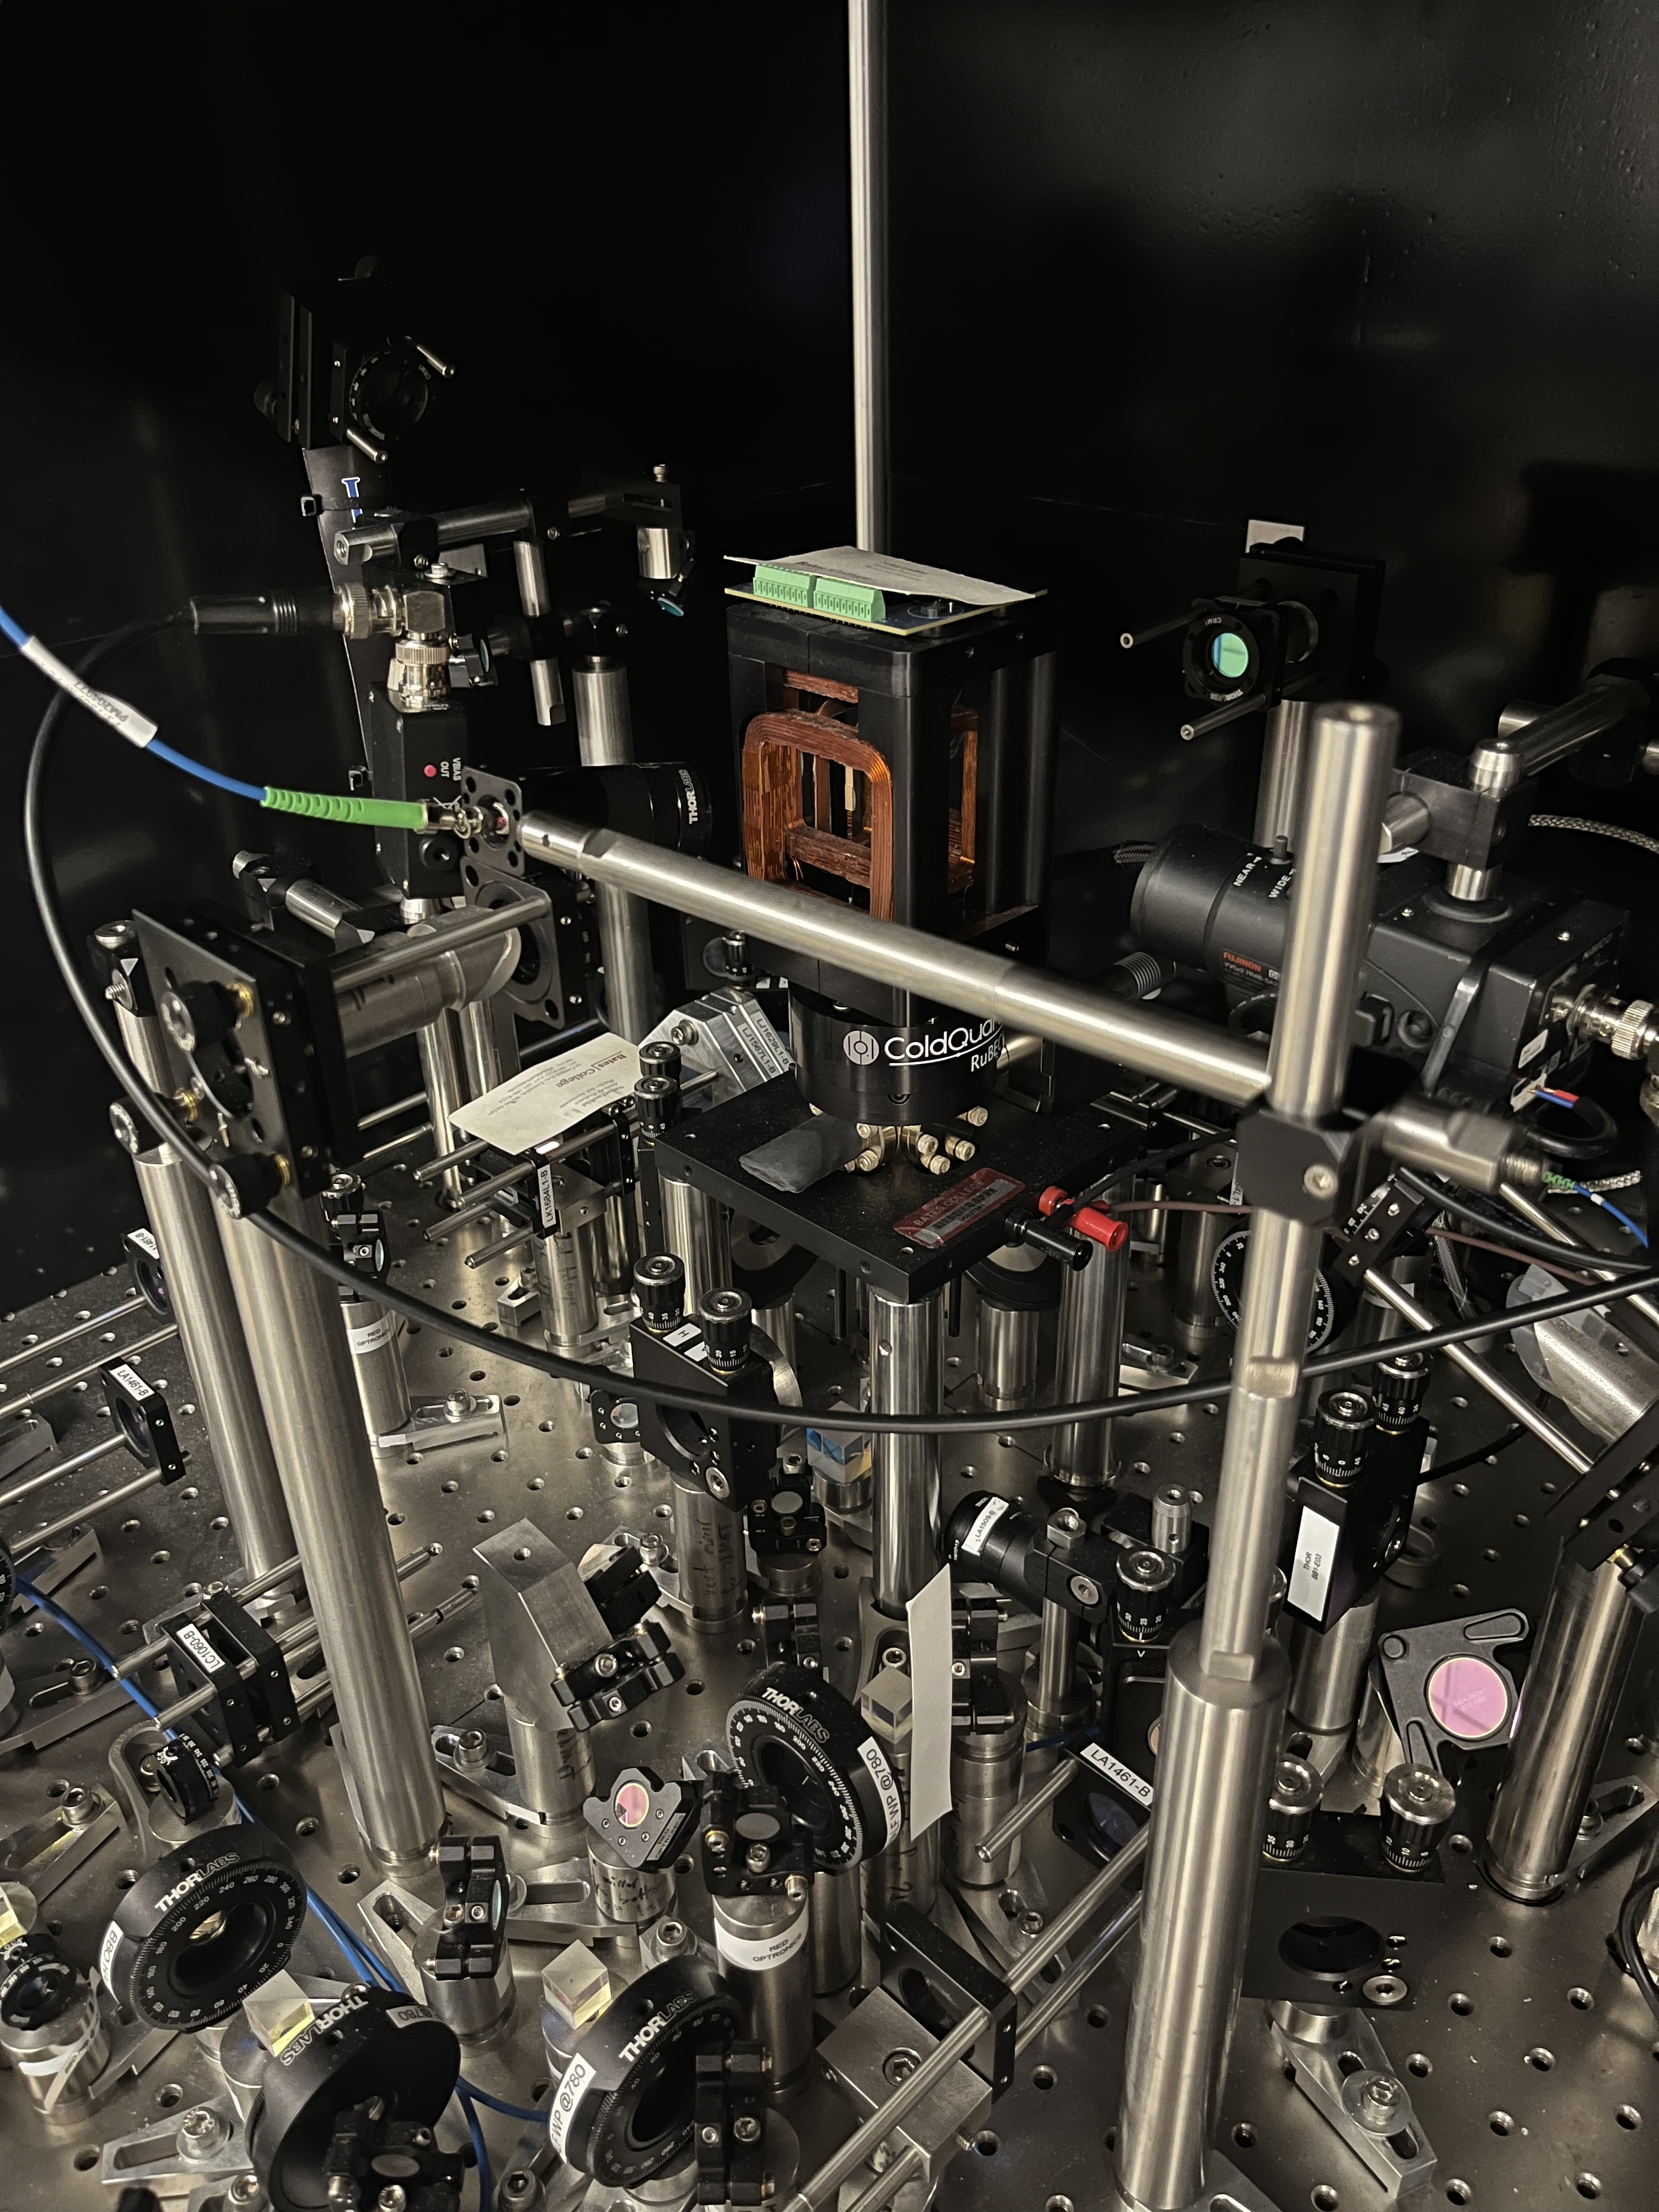
\epsfig{file=fig_shine_on_bec.jpg, scale = .11}
\end{center}
\caption{The optical pumping laser light mounted right above a principle axes. }
\end{figure}

 \section{Creating Positive Circularly Polarized Light}
 It was during this process that the optical fiber, when unscrewing it, broke. For this reason, this section will detail the steps to circularly polarizing the light, checking that it is polarized, and finalizing the optical pumping process. 

 When the light comes from out of the optical fiber it is linearly polarized. A quarter-wave plate is used to circularly polarize it. This mechanism is described in \textbf{Chapter 1.2.3}. The magnetic field from the quadrupole coil setup can then be adjusted to account for the slight misalignment from the principle axes and to make sure the atoms see positive circularly polarized light. The quarter-wave plate must be aligned in a specific way with the linear polarized light to circularly polarize the most amount of light. 
 
 To check if the the light is circularly polarized, a setup that contains a quarter-wave plate followed by a half-wave plate is used. This analyzer is shown in \textbf{Figure 3.4}. 

  \begin{figure}[h!]
\begin{center}
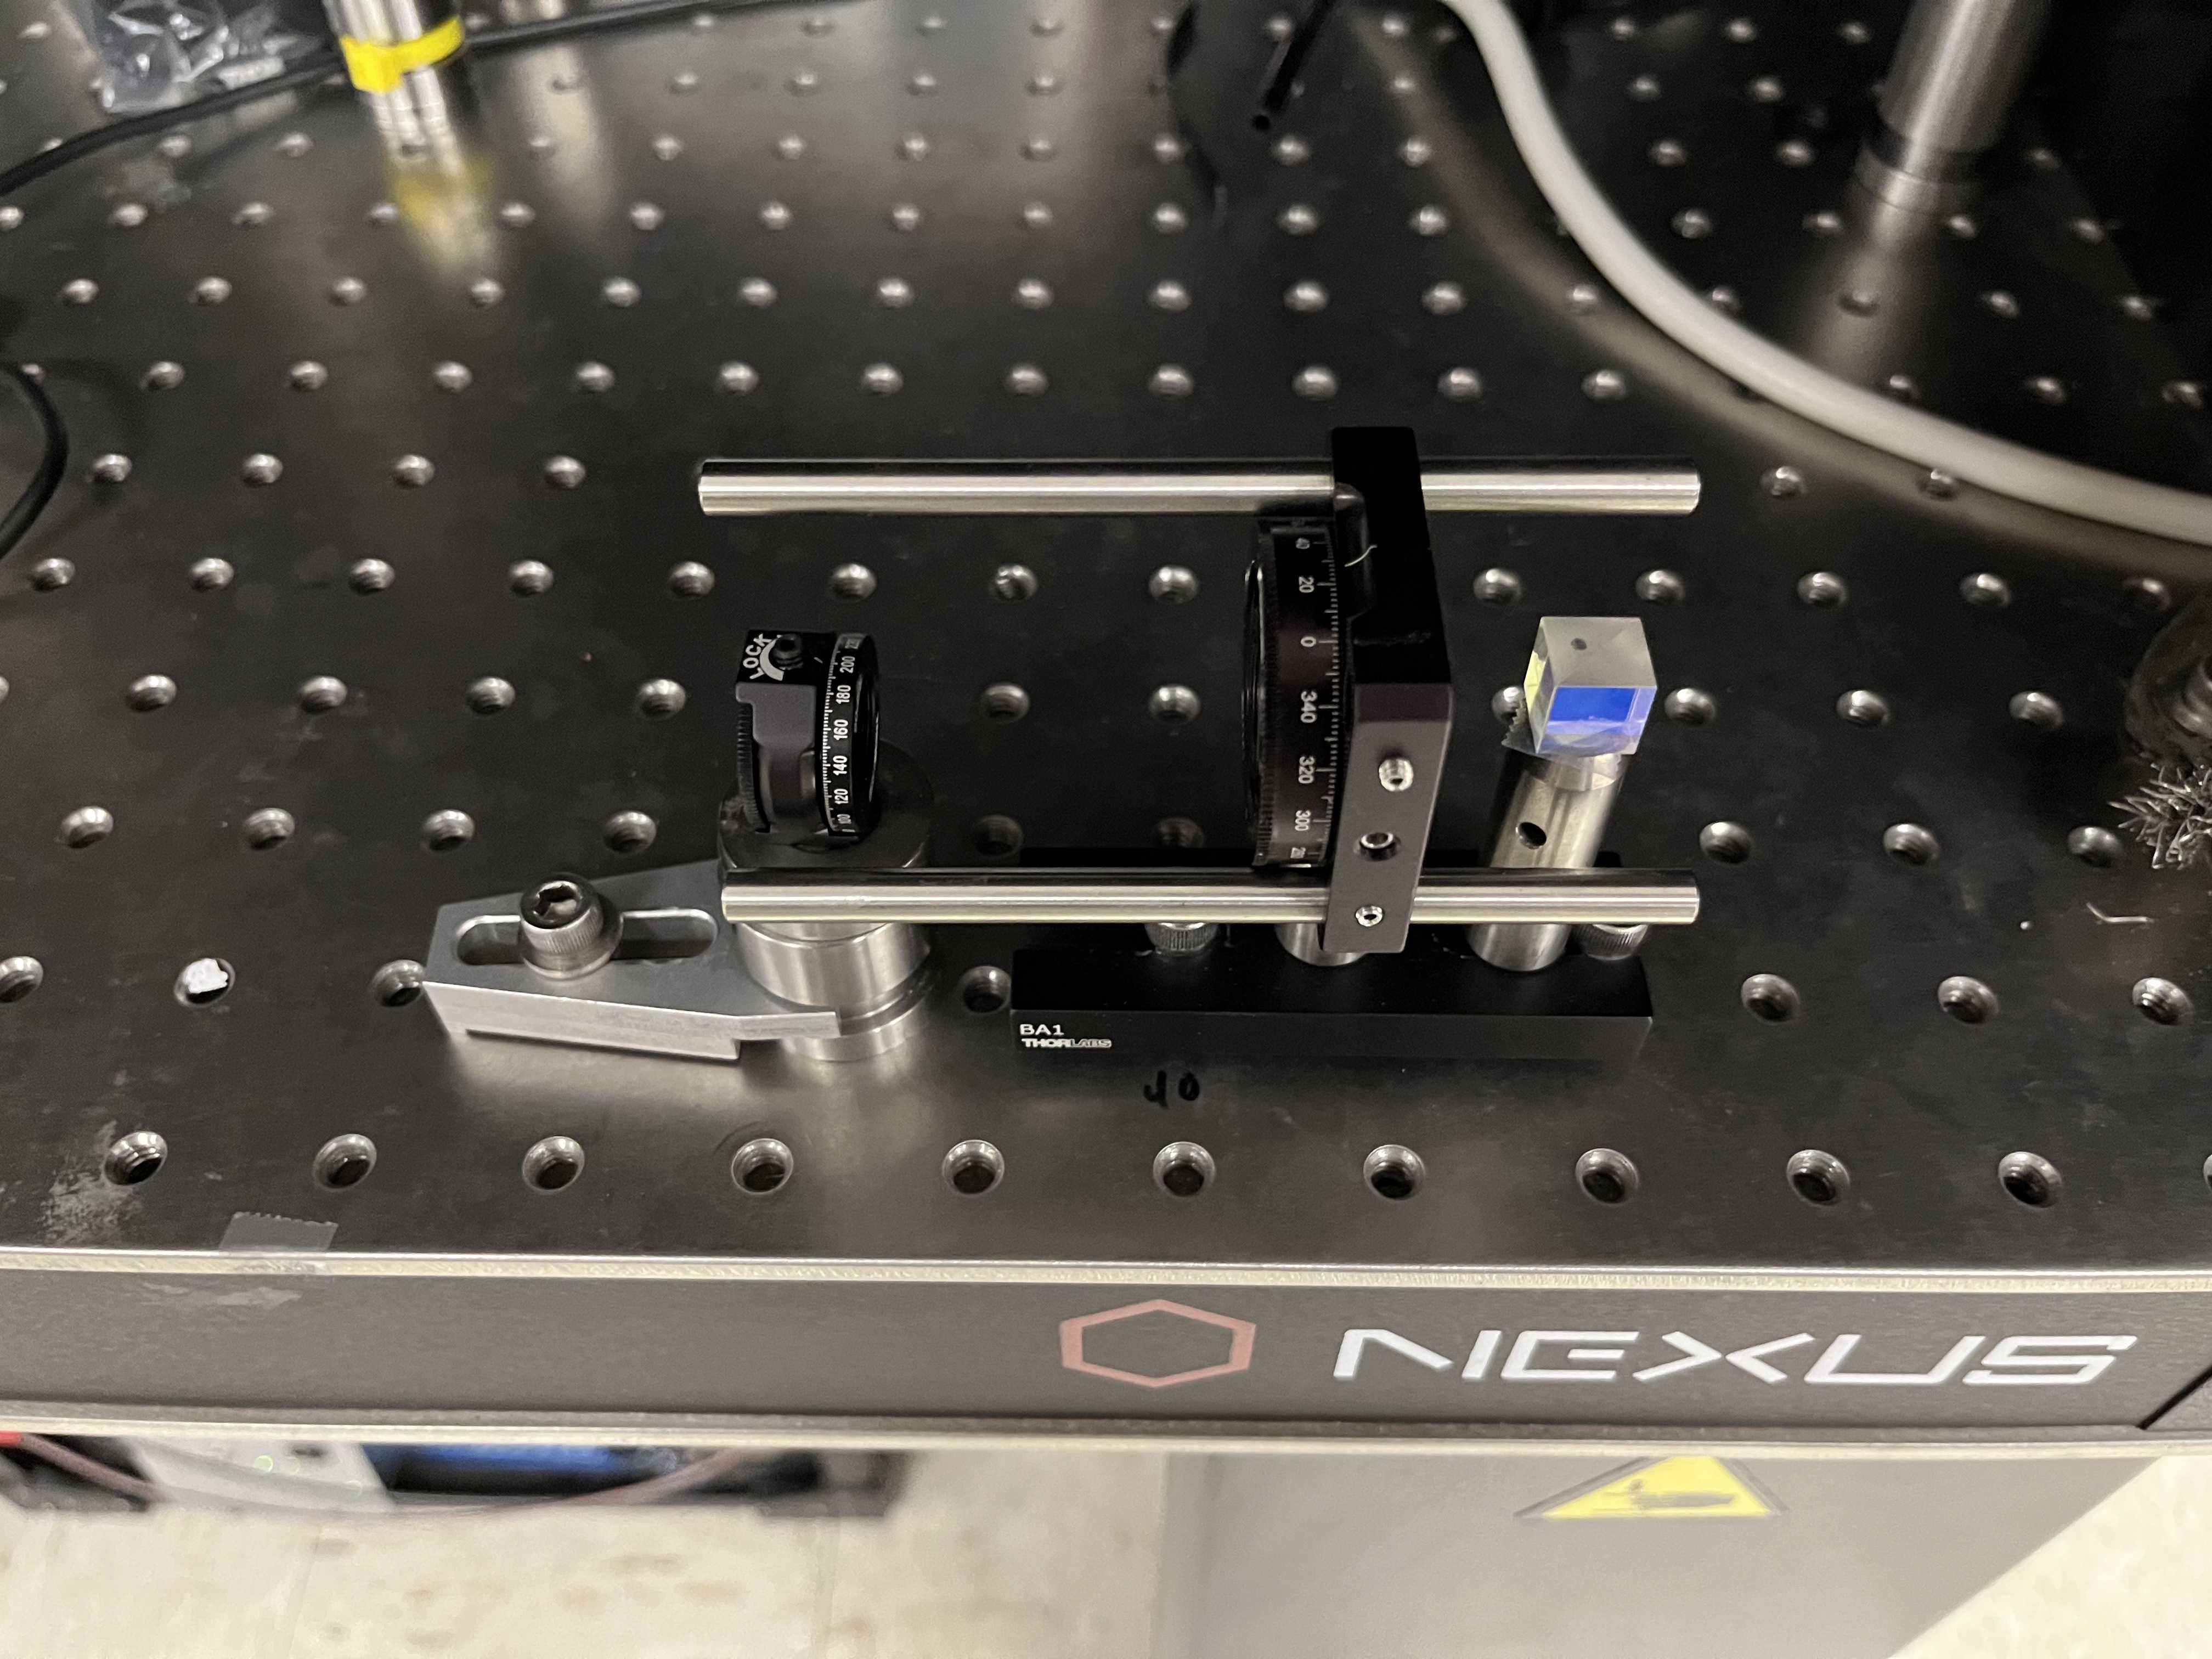
\epsfig{file=fig_polarizer_checker.jpg, scale = .11}
\end{center}
\caption{The circular polarizer analyzer. }
\end{figure}

The analyzer was clamped to the table for easy use by future students. The analyzer uses the quarter-wave plate to make the light linearly polarized. The half-wave plate is aligned so that nearly all the light will transmit through the beam splitter. If the light coming into the analyzer is not all circularly polarized, then the quarter-wave plate could circularly polarize some of it, and the half-wave plate and beam splitter will take the two orthogonal linear components of the light. This will result in a significant amount of light being reflected by the beam splitter. The student should shine the laser through this contraption and adjust the quarter-wave plate attached to the optical fiber so that as much light as possible is transmitted through the beam splitter. This is more efficiently done by minimizing the amount of light reflected by the beam splitter. These measurements are done with a power meter. 
\section{Future Steps}

A small cage mount was left for the next student. The lab should order a small cage mount that can hold the quarter-wave plate and turn to control its orientation, and of course another 10 meter optical fiber. This will make the process of mounting and checking the circular polarization easier. From there, the future steps are to create a LabVIEW process that can detune the laser and control the shutters for the optical pumping process. After that, the atoms should be caught in a magnetic trap and transferred to the chip for evaporative cooling. At that point, Bose-Einstein Condensation will be realized on the NASABEC machine. Finally, spectroscopy equipment can be used to observe the Bose-Einstein Condensate. 

\chapter*{Conclusion}
This thesis builds upon the work of other students and Nathan Lundblad. The thesis establishes a theory of quantum statistics of bosons and the formation of a state of matter known as Bose-Einstein Condensation. From there the typical steps followed for cooling atoms to temperatures of below $100nK$ are explained. These steps include forms of laser cooling, optical pumping and magnetic trapping, and finally evaporative cooling. This thesis then builds and describes a computational simulation of the optical pumping process. This program establishes a relationship between the desired proportion of trappable atoms and the number of photon scatters required per Rubidium atom. From there, \textbf{Equation 2.3} can be used to appropriately adjust the laser specifications. Lastly, the thesis describes the progress towards building an optical pumping set up for the NASABEC machine and outlines the next steps towards completing this process. 

Soon enough, with some dedicated students and hard work Bose-Einstein Condensation can be realized on the NASABEC machine. I'm \textit{pumped} to hear about it!













\nocite{*}
%
\section{Writing text in \LaTeX}
You can write text in \LaTeX ~ as you would in any other word processing or typesetting software.  You can incorporate \textit{different} \textbf{varieties} of \textsl{typeface}.  What's really exciting about writing text in \LaTeX 
~ is that it's very easy to incorporate weird symbols, like $\alpha$ or $\otimes$ or $\infty$ into your text.  Note that the weird symbols appear in between \$ signs -- this means that they occur in \textit{math mode}.

You create a new paragraph just by putting in a blank line.  Leaving extra space or extra lines in between paragraphs won't change their spacing at all.  \LaTeX ~ will automatically indent your paragraphs, so you don't have to worry about indenting.

\noindent You can, however prevent it from indenting your paragraphs if you'd like.  But that's getting a little ahead of ourselves.  

\section{Writing equations in \LaTeX}
It is beautifully easy to write equations, whether they occur inline with the text  $\Psi(x,t) = A e^{i(kx -\omega t)}$ or as a separate line
\begin{equation}
\Psi(x,t) =\sum_{n=1}^\infty c_n \psi_n(x) e^{-i E_n t/\hbar}.
\end{equation}
To continue a paragraph after an equation, make sure that there's no blank line between the equation and your next line of text.
Equations that are in a separate line will be numbered, and it's easy to refer to Eq.~\ref{SE} by labelling your equations  
\begin{equation}
i\hbar\frac{\partial}{\partial t}\Psi(x,t) = \hat{H} \Psi(x,t). 
\label{SE}
\end{equation}

Are you getting tired of writing begin\{eqnarray\} and end\{eqnarray\} yet?\footnote{Notice how I made a \} by putting a backslash in front of the symbol.  The curly brace has special meaning in \LaTeX, so if you want to make one, you have to let the program know that you want the symbol.}  You can simplify your life by defining abbreviated symbols for commands:
\newcommand{\beq}{\begin{equation}}
\newcommand{\eeq}{\end{equation}}
\beq
\langle x |\Psi(t)\rangle = \Psi(x,t).
\eeq
For simplicity, I'd suggest putting all of your new commands in a separate include file.

When writing a derivation with multiple steps, it is often useful to use an equation array
\begin{eqnarray}
\int_0^{2\pi}\sin^2{x}dx & = &  \int_0^{2\pi}\frac{1}{2}\left(1-\cos{2x}\right)dx \nonumber \\
& = & \left. \frac{1}{2}\left(x - \frac{\sin{2x}}{2}\right)\right|_0^{2\pi} \nonumber \\
& = & \pi. \nonumber 
\end{eqnarray}
Note that you can suppress equation numbering, which is often desirable in derivations!


The syntax for equation arrays is similar to the syntax for arrays within equations.  For example, 
\beq
\hat{H} = \left(\begin{array}{clcr}
		\Delta & \Omega & 0\\
		\Omega^*& 0 &\kappa \\
		0& \kappa^*&-\Delta\\ 
	\end{array}\right)
\eeq

There are many more complicated things you can do with equations, but this should be enough to get started! 

\section{Tables, lists, etc... etc...}
If you want to make a table, you'll need to specify the justification for each of the columns; \TeX will automatically calculate the column widths for you.  

\begin{table}[h]
\begin{center}
\begin{tabular}{|l|l|r|l|}
\hline
Name & Age & Town & Time \\
\hline
Joe Schmoe & 23 &  Rumford & 1:04\\
\hline
Mary Q. Contrary & 44 & Yarmouth & 1:12 \\
\hline
Baxter Boulevard & 32 & Portland & 1:42 \\
\hline
Lass Plaice & 60 & Lewiston & 1:57 \\
\hline
\end{tabular}
\caption{\label{raceresults}Not too many people showed up for the first, and probably last, annual Androscoggin swimming race.}
\end{center}
\end{table}

You might also, for example, want to 

\begin{enumerate}

\item make lists

\item number your lists

\end{enumerate}

\begin{itemize}

\item use bullet points

\item find better items to put in your bullet points

\end{itemize}

\section{Figures}

Figures are probably the hardest thing to do.  In order for these figures to show up, the figure files must be in the same folder as thesis.tex and all of your chapters.  

\begin{figure}[htbp] % float placement: (h)ere, page (t)op, page (b)ottom, other (p)age
  \centering
  % file name: C:/Users/home/Documents/Lily/Physics template/badfigure.eps
  \includegraphics[width=2.67in,height=3.51in,keepaspectratio]{badfigure}
  \caption{This is a very bad figure.}
  \label{fig:badfigure}
\end{figure}

If you are using .eps files for your figures, you can use the epsfig package, which is included at the very beginning of thesis.tex.
\begin{figure}[h]
\begin{center}
\epsfig{file=badfigure,height=8cm,width=12cm,angle=90}
\end{center}
\caption{A rescaled, stretched, and rotated bad figure.}
\end{figure}

\section{References}
While you can directly write a bibliography at the end of your .tex file, using BibTeX gives you much more freedom~\cite{chang2006}.  The .bib file includes all of your references, but only the ones you actually cite~\cite{JelezkoPrivate, Inui, Ernst, Ta} will appear in the bibliography, and you can easily alphabetize them, have them come in order of reference, and so on and so forth.  Use BibTeX!
%%stuff i might reuse

Over a large number of states, this summations becomes well approximated by a continuous integral.
\beq
N = \int_0^{\infty}{g(\epsilon)\frac{1}{e^{(\epsilon_s-\mu) /kT}-1}}d\epsilon
\eeq
where $g(\epsilon)$ is the density of the states, or the number of particle states per unit energy, calculated by summing the total energy from each electron. This density of states is inaccurate for very low temperatures. 
This integral yields the following
To distinguish at which temperature this occurs, a critical temperature is defined, $T_C$. 

https://physics.uwb.edu.pl/main/ptf/fizyka2000/bec/lascool4.html
https://www.google.com/url?sa=i&url=https%3A%2F%2Fwiki.physics.udel.edu%2Fwiki_phys813%2Fimages%2F2%2F28%2FBec_phys813.pdf&psig=AOvVaw2ku55eOWoUnkiEHhS_ddV1&ust=1681673016045000&source=images&cd=vfe&ved=0CBIQjhxqFwoTCMjh3qfOrP4CFQAAAAAdAAAAABAT

https://arxiv.org/ftp/physics/papers/0003/0003050.pdf

\backmatter
\chapter*{Appendix}
% The asterisk prevents this file from being labelled
% as a 'chapter.'
\section*{A.1 Bose-Einstein Distribution Derivation}
Starting with Equations 1.4 and 1.5, the average number of bosons occupying an energy state $s$ can be derived. 
\beq
P_s(n) = \frac{1}{\mathrm{Z}} e^{-n(\epsilon_s-\mu) /kT}\tag{1.4}
\eeq
\beq
\mathrm{Z}= \frac{1}{1- e^{-(\epsilon_s-\mu) /kT}}\tag{1.5}
\eeq
\begin{align*}
    \bar{n}_s = \sum_n{nP_s(n)} 
\end{align*}
For ease in notation, let's define a variable $x$, $x = \frac{(\epsilon_s-\mu) }{kT}$.
\begin{align*}
P_s(n) = \frac{1}{\mathrm{Z}} e^{-nx} 
\end{align*}
\begin{align*}
\bar{n}_s &= \sum_n{n\frac{1}{\mathrm{Z}} e^{-nx}}  \\
&= \frac{1}{\mathrm{Z}} \sum_n{ne^{-nx}} \\
&= -\frac{1}{\mathrm{Z}} \sum_n{\frac{\partial}{\partial x}e^{-nx}}
\end{align*}
As $\sum_n{}$ and $\frac{\partial}{\partial x}$ are both linear operators, they commute.
\begin{align*}
\bar{n}_s &=-\frac{1}{\mathrm{Z}} \frac{\partial}{\partial x}\sum_n{e^{-nx}} \\
\end{align*}
Under our new definition for $P_s(n)$, using $x= \frac{(\epsilon_s-\mu) }{kT}$, we find that 
\begin{align*}
    \Zeta &= \sum_n{e^{-nx}}
\end{align*}
Substituting this partition function into our equation for the average number of bosons in state $s$, we have created an expression for $\bar{n}_s$ that no longer contains an infinite sum. 
\begin{align*}
    \bar{n}_s &=-\frac{1}{\mathrm{Z}} \frac{\partial \Zeta}{\partial x}
\end{align*}
We can continue to solve using our previous definition for the partition function, substituting in $x = \frac{(\epsilon_s-\mu) }{kT}$
\beq
\mathrm{Z}= \frac{1}{1- e^{-(\epsilon_s-\mu) /kT}}\tag{1.5}
\eeq
\begin{align*}
    \mathrm{Z}&= \frac{1}{1- e^{-x}}\\
    \bar{n}_s &=-(1- e^{-x}) \frac{\partial }{\partial x}\left( \frac{1}{1- e^{-x}}\right) \\
    &= -(1- e^{-x}) (1- e^{-x})^{-2}(e^{-x})\\
    &= \frac{e^{-x}}{1-e^{-x}} \\
    &= \frac{1}{\frac{1}{e^{-x}}-1} \\
    \bar{n}_s  &= \frac{1}{e^x-1}\tag{1.6}
\end{align*}
The equation above is \textbf{Equation 1.6}, substituting in $x$. This equation is known as the Bose-Einstein distribution. 
\newpage

\section*{A.2 Rubidium-87 Energy Levels}

\begin{figure}[t]
\begin{center}
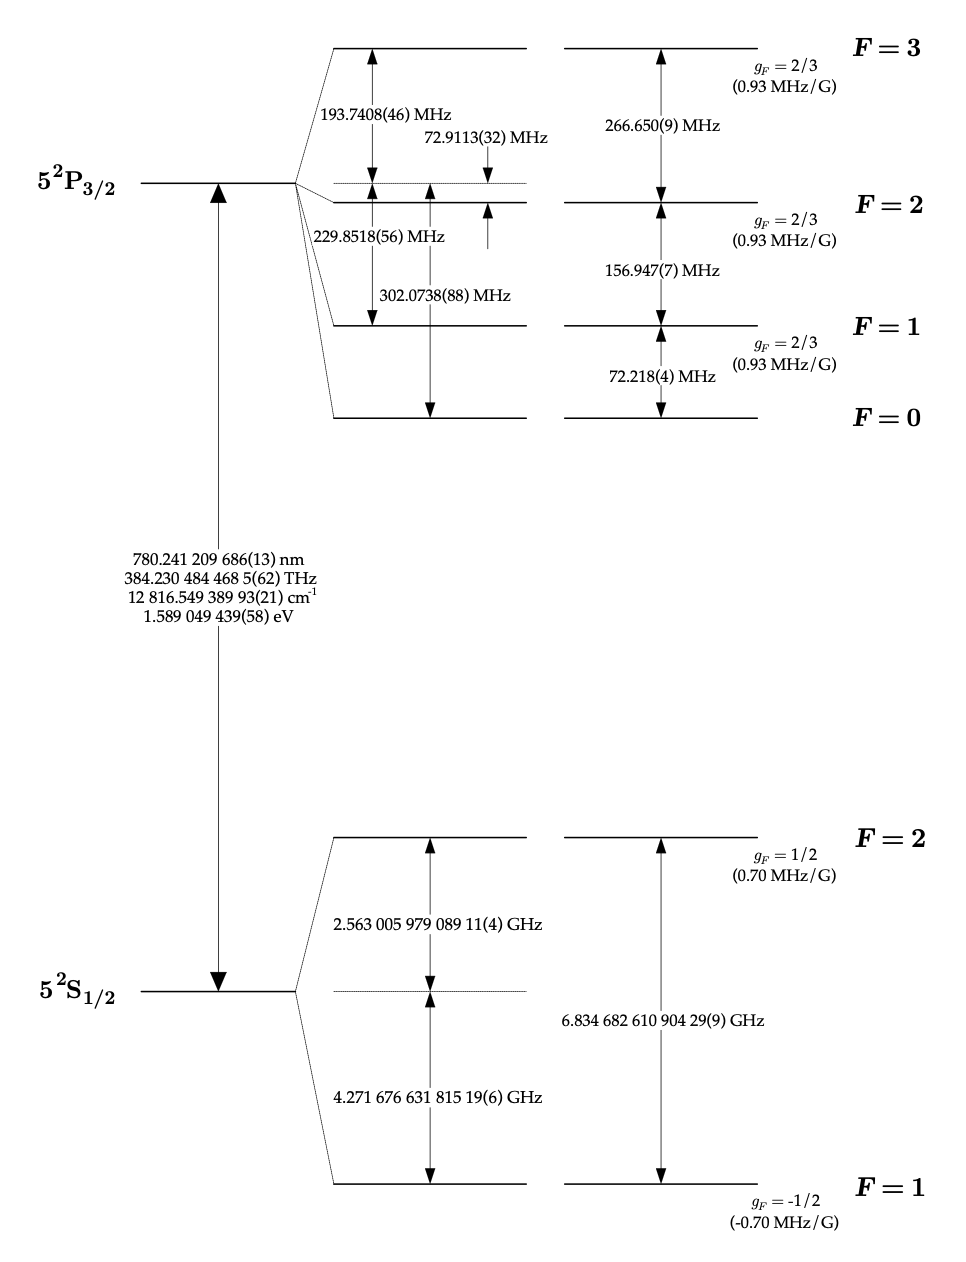
\epsfig{file=fig_rb_energy.png, scale = .9}
\end{center}
\end{figure}
\textbf{Figure A.1} The energy levels of Rubidium-87 and Land\'e factors. \cite{steck} 

\section*{A.3 Optical Pumping Simulation Code}
This code is written in python. 
\newline
\inputminted[fontsize=\footnotesize, frame=leftline, linenos]{python}{optical_pumping.py}

\endinput

			% Use \include{appendixB} to include another appendix.

\bibliographystyle{unsrt} %\bibliographystyle{plain} will put your references in alphabetical order by first author
\bibliography{biblio}
\end{document}
	
